\documentclass[sigconf,nonacm]{acmart}

%% Enable subfigures
\usepackage{subfigure}
%% Enable numbers in scientific format.
\usepackage{siunitx}
%% Enable enumerate start from.
\usepackage{enumitem}

%% Enable theorems
\newtheorem{theorem}{Theorem}[section]
\newtheorem{lemma}[theorem]{Lemma}

%% Enable algorithms
\usepackage{algorithm}
\usepackage[noend]{algpseudocode}
\let\ReturnInline\Return
\renewcommand{\Return}{\State\ReturnInline}
\algrenewcommand\algorithmicrequire{$\rhd$}
\algrenewcommand\algorithmicensure{$\square$}

%% Fonts used in the template cannot be substituted; margin 
%% adjustments are not allowed.
\AtBeginDocument{%
  \providecommand\BibTeX{{%
    \normalfont B\kern-0.5em{\scshape i\kern-0.25em b}\kern-0.8em\TeX}}}

%% Rights management information.
\setcopyright{acmcopyright}
\copyrightyear{2018}
\acmYear{2018}
\acmDOI{XXXXXXX.XXXXXXX}

%% These commands are for a PROCEEDINGS abstract or paper.
\acmConference[Conference acronym 'XX]{Make sure to enter the correct
  conference title from your rights confirmation emai}{June 03--05,
  2018}{Woodstock, NY}
%% Title of the proceedings is different from ``Proceedings of ...''?
% \acmBooktitle{Woodstock '18: ACM Symposium on Neural Gaze Detection,
%  June 03--05, 2018, Woodstock, NY} 
% \acmPrice{15.00}
% \acmISBN{978-1-4503-XXXX-X/18/06}

%% Submission ID.
% \acmSubmissionID{123-A56-BU3}

%% Use the "author year" style of citations and references?
% \citestyle{acmauthoryear}

%% Message
\newcommand{\kk}[1]{{{\color{red} #1}}}
\newcommand{\ds}[1]{{{\color{blue} #1}}}
\newcommand{\su}[1]{{{\color{green} #1}}}

%% Ignore block
\newcommand{\ignore}[1]{}

%% Macros
\newcommand{\Lou}{\textit{Louvain}}
\newcommand{\LPA}{\textit{LPA}}
\newcommand{\Hyb}{\textit{Hybrid Louvain-LPA}}
\newcommand{\Sta}{\textit{Static}}
\newcommand{\Nai}{P-ND}
\newcommand{\DelOrg}{\textit{$\Delta$-screening}}
\newcommand{\Del}{P-DDS}
\newcommand{\Fro}{P-DF}
\newcommand{\StaLou}{\textit{Static Louvain}}
\newcommand{\NaiLou}{$\text{P-ND}_\text{L}$}
\newcommand{\DelLou}{$\text{P-DDS}_\text{L}$}
\newcommand{\FroLou}{$\text{P-DF}_\text{L}$}
\newcommand{\StaLPA}{\textit{Static LPA}}
\newcommand{\NaiLPA}{$\text{P-ND}_\text{LPA}$}
\newcommand{\DelLPA}{$\text{P-DDS}_\text{LPA}$}
\newcommand{\FroLPA}{$\text{P-DF}_\text{LPA}$}
\newcommand{\FroHyb}{$\text{P-DF}_\text{H}$}




\begin{document}

%% Full title of the paper.
\title[DF-Louvain: Fast Incrementally Expanding Approach for Community Detection on Dynamic Graphs]{DF-Louvain: Fast Incrementally Expanding Approach for Community Detection on Dynamic Graphs}

%% Short title to be used in page headers (optional).
% \title[short title]{full title}
% \subtitle{Something other than the title}

%% Authors and their affiliations.
\author{Subhajit Sahu}
\email{subhajit.sahu@research.iiit.ac.in}
\affiliation{%
  \institution{IIIT Hyderabad}
  \streetaddress{Professor CR Rao Rd, Gachibowli}
  \city{Hyderabad}
  \state{Telangana}
  \country{India}
  \postcode{500032}
}

%% Concise author list in page headers.
%\renewcommand{\shortauthors}{Sahu, Kothapalli, and Banerjee, et al.}

%% Show page numbers.
\settopmatter{printfolios=true}

%% Short summary of the work to be presented in the article.
\begin{abstract}
Community detection is the problem of recognizing natural divisions in networks. A relevant challenge in this problem is to find communities on rapidly evolving graphs. This calls for designing dynamic algorithms that reuse earlier output, only process vertices likely to change their community, extract parallelism by processing a batch of updates, and have low overhead.

This paper addresses the design of a high-speed community detection algorithm in the batch dynamic setting. First, our optimized parallel implementations of the \textit{Louvain} and \textit{LPA} algorithms is presented. These implementations identify communities in $6.2$ seconds and $2.7$ seconds, respectively, on a single 64-core CPU, when processing an undirected web graph with $1.9$ billion edges. Next, our \textit{Dynamic Frontier} approach is discussed. Given a batch update of edge deletion and insertions, this approach incrementally identifies an approximate set of affected vertices in the graph is with minimal overhead. We apply this approach to both \textit{Louvain}, a high quality, and \textit{Label Propagation Algorithm (LPA)}, a high speed static community detection algorithm. Our approach achieves a mean speedup of $1.5\times$ and $10.0\times$ when applied to \textit{Louvain} and \textit{LPA} respectively, compared to the best of two other dynamic approaches. Finally, we show how to combine \textit{Louvain} and \textit{LPA} with the \textit{Dynamic Frontier} approach to arrive at a novel hybrid algorithm. This algorithm produces high-quality communities while providing a speedup of $7.5\times$ on top of \textit{Dynamic Frontier} based \textit{Louvain}.
\end{abstract}

%% The code below is generated by the tool at http://dl.acm.org/ccs.cfm.
\begin{CCSXML}
<ccs2012>
<concept>
<concept_id>10003752.10003809.10010170</concept_id>
<concept_desc>Theory of computation~Parallel algorithms</concept_desc>
<concept_significance>500</concept_significance>
</concept>
<concept>
<concept_id>10003752.10003809.10003635</concept_id>
<concept_desc>Theory of computation~Graph algorithms analysis</concept_desc>
<concept_significance>500</concept_significance>
</concept>
</ccs2012>
\end{CCSXML}

% \ccsdesc[500]{Theory of computation~Parallel algorithms}
% \ccsdesc[500]{Theory of computation~Graph algorithms analysis}

%% Pick words that accurately describe the work being presented.
\keywords{Community detection, Parallel Louvain algorithm}

% \received{20 February 2007}
% \received[revised]{12 March 2009}
% \received[accepted]{5 June 2009}



%% Process the author and title information.
\maketitle

\section{Introduction}
\label{sec:introduction}
Identifying hidden communities within networks is a crucial graph analytics problem that arises in various domains such as drug discovery, disease prediction, protein annotation, topic discovery, inferring land use, and criminal identification. Here, we want to identify groups of vertices that exhibit dense internal connections but sparse connections with the rest of the graph. One of the difficulties in the community detection problem is the lack of apriori knowledge on the number and size distribution of communities. These communities are intrinsic when identified based on network topology alone, without external attributes, and they are disjoint when each vertex belongs to only one community \cite{com-gregory10}. However, the problem is NP-hard, and there is a lack of apriori knowledge on the number and size distribution of communities \cite{com-blondel08}. To solve this issue, researchers have come up with a number of heuristics for finding communities \cite{com-guimera05, com-derenyi05, com-newman06, com-reichardt06, com-raghavan07, com-blondel08, com-rosvall08, infomap-rosvall09, com-fortunato10, com-gregory10, com-kloster14, com-come15, com-ruan15, com-newman16, com-ghoshal19, com-rita20, com-lu20, com-gupta22}. To measure the quality of communities identified, fitness metrics such as the modularity score proposed by Newman et al. \cite{com-newman06} are used.\ignore{Normalized Mutual Information index (NMI) \cite{com-jain17, com-chopade17}, and Jaccard Index \cite{com-jain17} are also employed.}

The \textit{Louvain method}, proposed by Blondel et al. \cite{com-blondel08}, is one of the most popular community detection algorithms \cite{com-lancichinetti09}. It is a greedy, modularity-based optimization algorithm, that hierarchically agglomerates vertices in a graph to obtain communities \cite{com-blondel08}. It has a time complexity of $O(KM)$\ignore{and an average time complexity of $\Theta (N \log N)$} (where $M$ represents the number of edges in the graph, $K$ the total number of iterations performed across all passes), and it efficiently identifies communities with resulting high modularity. A number of algorithmic improvements to the Louvain algorithm have been proposed \cite{com-rotta11, com-waltman13, com-gach14, com-ryu16, com-ozaki16, com-traag15, com-lu15, com-naim17, com-halappanavar17, com-ghosh18, com-traag19, com-shi21, com-zhang21, com-you22, com-aldabobi22}. To parallelize the algorithm on multicore CPUs \cite{staudt2015engineering, staudt2016networkit, com-fazlali17, com-halappanavar17, qie2022isolate}, GPUs \cite{com-naim17}, CPU-GPU hybrids \cite{com-bhowmik19, com-mohammadi20}, multi-GPUs \cite{com-cheong13, hricik2020using, chou2022batched, com-gawande22}, and multi-node systems \cite{com-ghosh18, ghosh2018scalable, sattar2022scalable, com-bhowmick22}, a number of strategies have been attempted \cite{com-cheong13, com-wickramaarachchi14, com-zeng15, com-que15, com-fazlali17, com-naim17, com-halappanavar17, com-ghosh18, com-bhowmik19, com-mohammadi20, com-shi21, com-bhowmick22}.

However, many real-world graphs rapidly evolve with time, through the insertion/deletion of edges/vertices. These graphs are usually immense in scale, stemming from applications such as machine learning and social networks, and are gradually becoming ubiquitous.\ignore{With this data deluge, newer challenges are emerging.} For efficiency reasons, one needs algorithms that update the results without re-computing from scratch. Such algorithms are known as \textit{dynamic algorithms}. Parallel algorithms for graph analytics on dynamic graphs have thus become a subject of considerable research interest. Examples of parallel dynamic algorithms include those for dynamic graph coloring \cite{color-yuan17, color-bhattacharya18}, maintaining shortest routes \cite{path-zhang17, path-khanda21}, and updating centrality scores \cite{cent-shao20, cent-regunta21}.

A growing number of research efforts have focused on detecting communities in dynamic networks. The goal of dynamic community detection is to obtain high-quality communities while minimizing computation time. A suitable dynamic community detection approach should find an approximate affected set of vertices that covers most of the true affected set of vertices as possible (too small and we get bad communities, too large and we increase computation time), while requiring the least amount of time (overhead) \cite{incr-ramalingam96}. Note that if the subset of the graph identified as \textit{affected} is too small, we may end up with inaccurate communities, and if the subset is too large, we incur a significant computation time. Hence, one should look to identify the appropriate set of affected vertices. In addition, determining the vertices to be processed should have low overhead \cite{incr-ramalingam96}.

\ignore{The simplest approach for dynamic community detection is to use the community membership of vertices from the previous snapshot of the graph \cite{com-aynaud10, com-chong13, com-shang14, com-zhuang19} (which we call \textit{Naive-dynamic}). Alternatively, more advanced techniques have been employed to minimize computation by identifying a smaller subset of the graph that is affected by changes, such as moving only changed vertices \cite{com-aktunc15, com-yin16}, recomputing vertices close to an updated edge (below a given threshold distance) \cite{com-held16}, disbanding affected communities to lower-level network \cite{com-cordeiro16}, or using a dynamic modularity metric to compute community membership of vertices from scratch \cite{com-meng16}. \textit{Delta-Screening} (or \textit{$\Delta$-screening}) is a recently proposed technique that finds a subset of vertices impacted by changes in a graph using delta-modularity \cite{com-zarayeneh21}.}

However, a critical examination of the extant literature on dynamic community detection algorithms indicates a few shortcomings. Some of these algorithms \cite{com-cordeiro16, com-meng16} do not outperform static algorithms even for modest-sized batch updates. Aynaud et al. \cite{com-aynaud10} and Chong et al. \cite{com-chong13} adapt the existing community labels and run an algorithm, such as Louvain, on the entire graph. Often, this is unwarranted since not every vertex would need to change its community on the insertion/deletion of a few edges. Cordeiro et al. \cite{com-cordeiro16} do not consider the cascading impact of changes in community labels, where the community label of a vertex changes because of a change in the community label of its neighbor. Zarayeneh et al. \cite{com-zarayeneh21} identify a subset of vertices whose community labels are likely to change on the insertion/deletion of a few edges. However, as this set of vertices identified is large, the algorithm of Zaranayeh et al. incurs a significant computation time. Moreover, most of the reported algorithms \cite{com-aynaud10, com-chong13, com-meng16, com-cordeiro16, com-zhuang19, com-zarayeneh21} are sequential. There is thus a pressing need for efficient parallel algorithms for community detection on large dynamic graphs. Further, none of the works recommend reusing the previous \textit{total edge weight} of each vertex/community (required for local-moving phase of Louvain algorithm) as auxiliary information to the dynamic algorithm. Recomputing it from scratch is expensive and becomes a bottleneck for dynamic Louvain algorithm. Table \ref{tab:compare} summarizes the above discussion.

\begin{table}[hbtp]
  \centering
  \caption{Speedup of our multicore implementation of Leiden algorithm compared to other state-of-the-art implementations. Direct comparisons entail running the given implementation on our server, while indirect comparisons (marked with a $*$, explained in Section \ref{sec:comparison-indirect}) involve comparing results relative to a common reference\ignore{(original Leiden)}.\ignore{Notably, the Leiden implementations vary in their classification, with some being multi-core and others multi-node.}}
  \label{tab:compare}
  \begin{tabular}{|c|c||c|}
    \toprule
    \textbf{Leiden implementation} &
    \textbf{Published} &
    \textbf{Our Speedup} \\
    \midrule
    Static \cite{sahu2023gvelouvain} & 2023 & $22\times$ \\ \hline
    Naive-dynamic \cite{csardi2006igraph} & 2006 & $\gg 50\times$ \\ \hline
    Delta-screening \cite{com-zarayeneh21} & 2021 & $\gg 20\times$ \\ \hline
    DynaMo \cite{com-zhuang19} & 2019 & $\gg 166\times^*$ \\ \hline
    Batch \cite{com-chong13} & 2013 & $\gg 22\times^*$ \\ \hline
  \bottomrule
  \end{tabular}
\end{table}





\subsection{Our Contributions}

This paper addresses the design of an efficient Parallel Louvain algorithm in the batch dynamic setting, where multiple edge updates are processed simultaneously. We first discuss our Dynamic Frontier (DF) approach that incrementally identifies an approximate set of affected vertices in the graph, given a batch of edge deletions and insertions, with low runtime overhead. In addition to accepting the previous community membership of each vertex, our algorithm accepts the previous total edge weight of each vertex as auxiliary information in order to improve scalability. We then show how to combine our DF approach with the Louvain method. We compare DF with two other dynamic approaches, the Naive-dynamic (ND) approach, and the $\Delta$-screening ($\Delta S$) approach. On a collection of $12$ graphs from four different classes, our experiments indicate that DF Louvain has a mean improved performance of $1.5\times$ compared to ND Louvain, while obtaining communities of the same quality. The work presented by Zarayeneh et al. \cite{com-zarayeneh21} demonstrates improved performance of $\Delta$-screening compared to Dynamo \cite{com-zhuang19} and Batch \cite{com-chong13}. As the DF approach outperforms $\Delta$-screening, we expect similar gains compared to Dynamo and Batch. Further, unlike Static Louvain, which may change significantly the way communities are obtained between snapshots (two runs in the snapshot lead to different solutions due its non-determinism), in our proposed algorithm, unaffected communities keep unchanged, i.e., they preserve the same nodes and even the same community id between snapshots. Community stability is important because it will simplify the process of tracking of communities over time. We show that our algorithm achieves \textit{good} community stability. Finally, we show that our algorithm has good scaling performance.




%% - Use --- for a dash.
%% - Use ``camera-ready'' for quotes.
%% - Use {\itshape very} or \textit{very} for italicized text.
%% - Use \verb|acmart| or {\verb|acmart|} for mono-spaced text.
%% - Use \url{https://capitalizemytitle.com/} for URLs.
%% - Use {\bfseries Do not modify this document.} for important boldface details.
%% - Use \ref{fig:name} for referencing.

%% For a block of pre-formatted text: 
% \begin{verbatim}
%   \renewcommand{\shortauthors}{McCartney, et al.}
% \end{verbatim}

%% For a list of items:
% \begin{itemize}
% \item the ``ACM Reference Format'' text on the first page.
% \item the ``rights management'' text on the first page.
% \item the conference information in the page header(s).
% \end{itemize}

%% For a table:
% \begin{table}
%   \caption{Frequency of Special Characters}
%   \label{tab:freq}
%   \begin{tabular}{ccl}
%     \toprule
%     Non-English or Math&Frequency&Comments\\
%     \midrule
%     \O & 1 in 1,000& For Swedish names\\
%     $\pi$ & 1 in 5& Common in math\\
%     \$ & 4 in 5 & Used in business\\
%     $\Psi^2_1$ & 1 in 40,000& Unexplained usage\\
%   \bottomrule
% \end{tabular}
% \end{table}

%% For a full-width table:
% \begin{table*}
%   \caption{Some Typical Commands}
%   \label{tab:commands}
%   \begin{tabular}{ccl}
%     \toprule
%     Command &A Number & Comments\\
%     \midrule
%     \texttt{{\char'134}author} & 100& Author \\
%     \texttt{{\char'134}table}& 300 & For tables\\
%     \texttt{{\char'134}table*}& 400& For wider tables\\
%     \bottomrule
%   \end{tabular}
% \end{table*}


%% For inline math:
% \begin{math}
%   \lim_{n\rightarrow \infty}x=0
% \end{math},

%% For a numbered equation:
% \begin{equation}
%   \lim_{n\rightarrow \infty}x=0
% \end{equation}

%% For an unnumbered equation:
% \begin{displaymath}
%   \sum_{i=0}^{\infty} x + 1
% \end{displaymath}

%% For a figure:
% \begin{figure}[h]
%   \centering
%   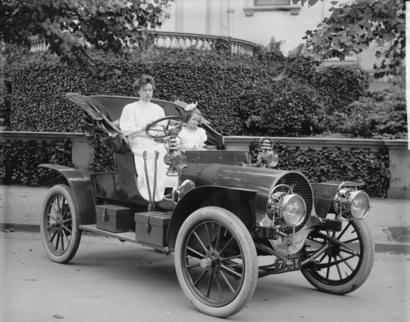
\includegraphics[width=\linewidth]{inc/sample-franklin}
%   \caption{1907 Franklin Model D roadster. Photograph by Harris \&
%     Ewing, Inc. [Public domain], via Wikimedia
%     Commons. (\url{https://goo.gl/VLCRBB}).}
%   \Description{A woman and a girl in white dresses sit in an open car.}
% \end{figure}

%% For a teaser figure.
% \begin{teaserfigure}
%   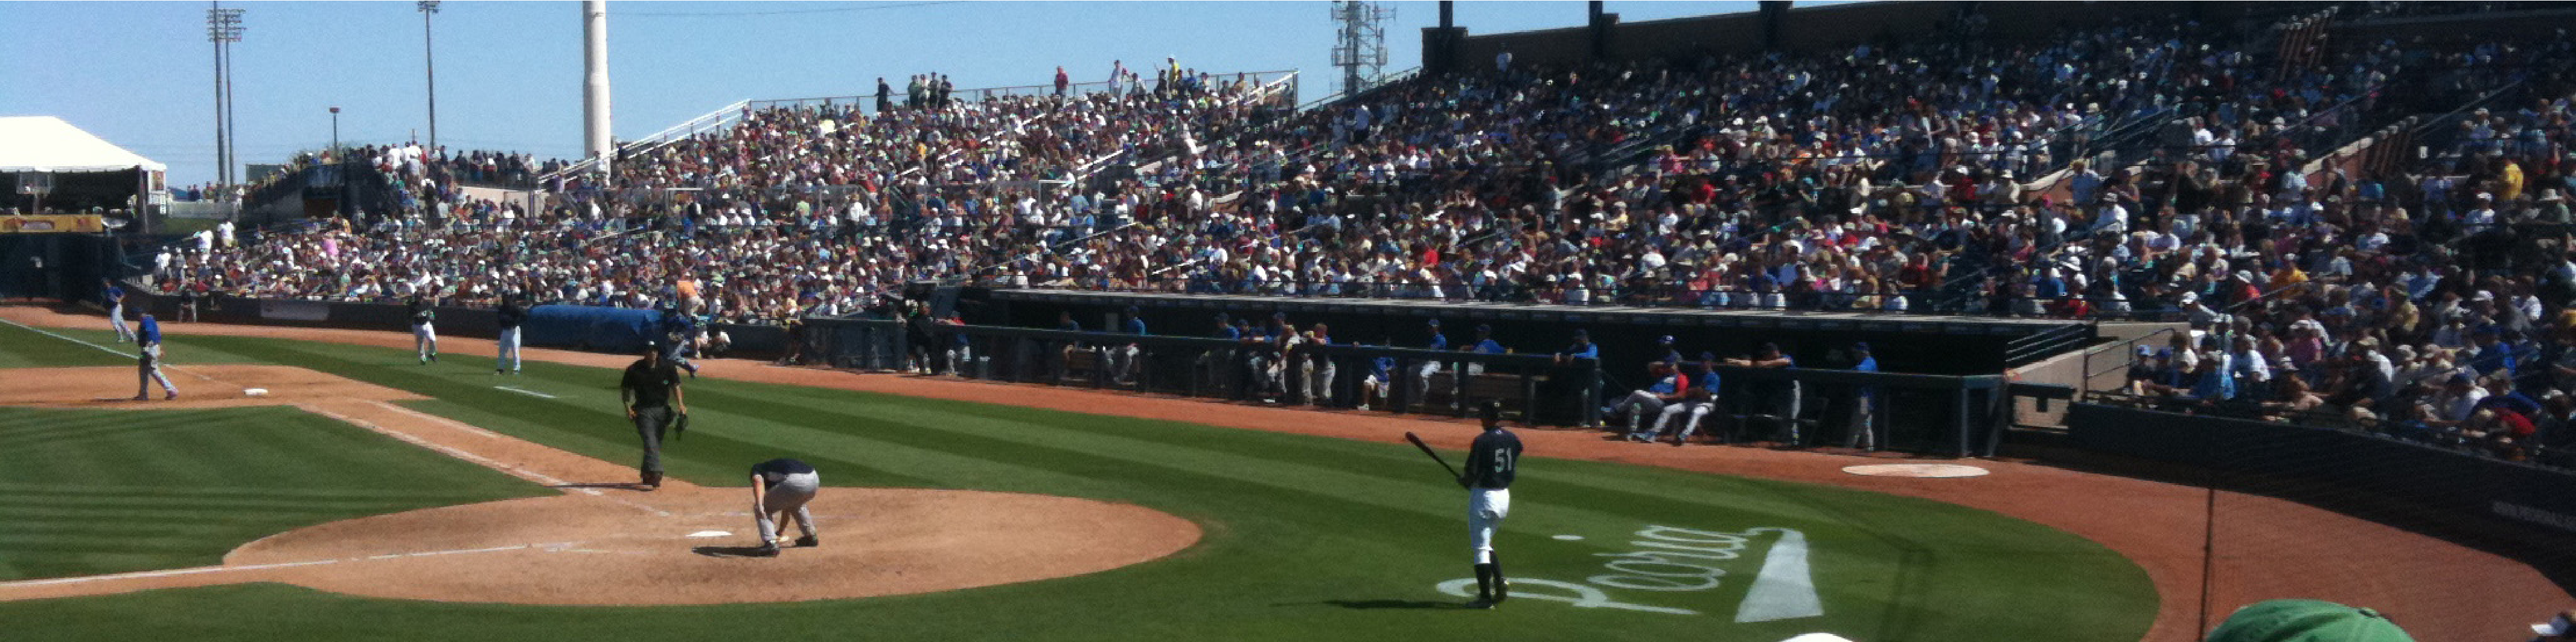
\includegraphics[width=\textwidth]{sampleteaser}
%   \caption{figure caption}
%   \Description{figure description}
% \end{teaserfigure}


\section{Related work}
\label{sec:related}
Identifying hidden communities within networks is a crucial graph analytics problem that arises in various domains such as drug discovery, disease prediction, protein annotation, topic discovery, inferring land use, and criminal identification. The main objective is to identify groups of vertices that exhibit dense internal connections but sparse connections with the rest of the graph \cite{com-gregory10}. However, this problem is NP-hard, and there is a lack of apriori knowledge on the number and size distribution of communities \cite{com-blondel08}.

To solve this issue, researches have come up with a number of heuristics for finding communities. These include label propagation \cite{com-raghavan07, com-gregory10}, random walk \cite{com-rosvall08}, diffusion \cite{com-kloster14}, spin dynamics \cite{com-reichardt06}, fitness metric optimization \cite{com-newman06, com-fortunato10}, statistical inference \cite{com-come15, com-newman16}, core clustering \cite{com-ruan15}, simulated annealing \cite{com-guimera05, com-reichardt06}, clique percolation \cite{com-derenyi05, com-gupta22}, information theory (infomap) \cite{infomap-rosvall09, com-rita20}, and  biological evolution (genetics) \cite{com-ghoshal19, com-lu20} are studied over the decades for this problem. To evaluate the success of these methods, metrics such as the modularity score \cite{com-newman06, com-blondel08}, Normalized Mutual Information index (NMI) \cite{com-jain17, com-chopade17}, and Jaccard Index \cite{com-jain17} are often employed.

The \textit{Louvain} algorithm, based on modularity optimization, employs a greedy strategy to hierarchically merge graph vertices and extract communities \cite{com-blondel08}. It has a time complexity of $O(KM)$ (where $M$ represents the number of edges in the graph, $K$ represents the total number of iterations performed across all passes), and it efficiently identifies communities with resulting high modularity. As a result, the \textit{Louvain} method is widely favored among researchers \cite{com-lancichinetti09}.

Algorithmic improvements to the original algorithm have been proposed, which include early pruning of non-promising candidates (leaf vertices) \cite{com-ryu16, com-halappanavar17, com-zhang21, com-you22}, attempting local move only on likely vertices \cite{com-ryu16, com-ozaki16, com-zhang21, com-shi21}, ordering of vertices based on node importance \cite{com-aldabobi22}, moving nodes to a random neighbor community \cite{com-traag15}, threshold scaling \cite{com-lu15, com-naim17, com-halappanavar17}, threshold cycling \cite{com-ghosh18}, subnetwork refinement \cite{com-waltman13, com-traag19}, multilevel refinement \cite{com-rotta11, com-gach14, com-shi21}, and early termination \cite{com-ghosh18},

To parallelize the algorithm on multicore CPUs, GPUs \cite{com-cheong13}, hybrid CPU-GPUs \cite{com-bhowmik19}, multi GPUs \cite{com-cheong13, com-gawande22, com-bhowmick22}, and distributed systems \cite{com-bhowmick22}, a number of strategies have been attempted. These include parallelizing the costly first iteration \cite{com-wickramaarachchi14}, performing iterations asynchronously \cite{com-que15, com-shi21}, ordering vertices via graph coloring \cite{com-halappanavar17}, using vector based hashtables \cite{com-halappanavar17}, using adaptive parallel thread assignment \cite{com-fazlali17, com-naim17, com-mohammadi20}, using sort-reduce instead of hashing \cite{com-cheong13}, using simple partitions based of vertex ids \cite{com-cheong13, com-ghosh18}, and identifying and moving ghost/doubtful vertices \cite{com-zeng15, com-que15, com-bhowmik19, com-bhowmick22}.

The \textit{Label Propagation Algorithm (LPA)} is a method used for identifying communities or groups within a network by initializing each vertex with a unique label and diffusing these labels across the graph. It is faster and more scalable than the Louvain algorithm, as it does not require repeated optimization steps and is easy to parallelize \cite{com-newman04, com-raghavan07}.

Improvements upon the LPA include using a stable (non-random) mechanism of label choosing in the case of multiple best labels \cite{com-xing14}, addressing the issue of monster communities \cite{com-berahmand18, com-sattari18}, identifying central nodes and combining communities for improved modularity \cite{com-you20}, and using frontiers with alternating push-pull to reduce the number of edges visited and improve solution quality \cite{com-liu20}. A GPU-accelerated parallel implementation of the original LPA is available that is able to deal with large-scale datasets that do not fit into GPU memory \cite{com-kozawa17}.

A growing number of research efforts have focused on detecting communities in dynamic networks. The simplest approach is to use the community membership of vertices from the previous snapshot of the graph \cite{com-aynaud10, com-chong13, com-shang14, com-zhuang19} (which we call \textit{Naive-dynamic}). Alternatively, more advanced techniques have been employed to minimize computation by identifying a smaller subset of the graph that is affected by changes, such as moving only changed vertices \cite{com-aktunc15, com-yin16}, recomputing vertices close to an updated edge (below a given threshold distance) \cite{com-held16}, disbanding affected communities to lower-level network \cite{com-cordeiro16}, or using a dynamic modularity metric to compute community membership of vertices from scratch \cite{com-meng16}. \textit{Delta-Screening} (or \textit{$\Delta$-screening}) is a recently proposed technique that finds a subset of vertices impacted by changes in a graph using delta-modularity \cite{com-zarayeneh21}.

Significant research effort has also been dedicated to the development of dynamic label-propagation methods, due to their simplicity, efficiency, and scalability. In addition to the \textit{Naive-dynamic} approach, a number of advanced techniques been proposed. These include using the MapReduce model to efficiently adjust the communities of certain vertices based on previous intervals \cite{com-li17}, and using a stabilized label propagation process based on the static LabelRank algorithm \cite{com-xie13}. Adaptive Label Propagation Algorithm (ALPA) is another dynamic approach, which first performs a warm-up LPA on a subset of the network determined by edge deletions and insertions, followed by Local Label Propagation (LLP) which expands as a frontier of nodes that change labels and removes nodes that do not change labels \cite{com-han17}.


\section{Preliminaries}
\label{sec:preliminaries}
Let $G(V, E, w)$ be an undirected graph, with $V$ as the set of vertices, $E$ as the set of edges, and $w_{ij} = w_{ji}$ a positive weight associated with each edge in the graph. If the graph is unweighted, we assume each edge to be associated with unit weight ($w_{ij} = 1$). Further, we denote the neighbors of each vertex $i$ as $J_i = \{j\ |\ (i, j) \in E\}$, the weighted degree of each vertex $i$ as $K_i = \sum_{j \in J_i} w_{ij}$, the total number of vertices in the graph as $N = |V|$, the total number of edges in the graph as $M = |E|$, and the sum of edge weights in the undirected graph as $m = \sum_{i, j \in V} w_{ij}/2$.




\subsection{Community detection}

Disjoint community detection is the process of arriving at a community membership mapping, $C: V \rightarrow \Gamma$, which maps each vertex $i \in V$ to a community-id $c \in \Gamma$, where $\Gamma$ is the set of community-ids. We denote the vertices of a community $c \in \Gamma$ as $V_c$. We denote the community that a vertex $i$ belongs to as $C_i$. Further, we denote the neighbors of vertex $i$ belonging to a community $c$ as $J_{i \rightarrow c} = \{j\ |\ j \in J_i\ and\ C_j = c\}$, the sum of those edge weights as $K_{i \rightarrow c} = \{w_{ij}\ |\ j \in J_{i \rightarrow c}\}$, the sum of weights of edges within a community $c$ as $\sigma_c = \sum_{(i, j) \in E\ and\ C_i = C_j = c} w_{ij}$, and the total edge weight of a community $c$ as $\Sigma_c = \sum_{(i, j) \in E\ \mbox{and}\ C_i = c} w_{ij}$ \cite{com-zarayeneh21, com-leskovec21}.




\subsection{Modularity}

Modularity is a fitness metric that is used to evaluate the quality of communities obtained by community detection algorithms (as they are heuristic based). It is calculated as the difference between the fraction of edges within communities and the expected fraction of edges if the edges were distributed randomly. It lies in the range $[-0.5, 1]$ (higher is better) \cite{com-brandes07}. Optimizing this function theoretically leads to the best possible grouping \cite{com-newman04, com-traag11}.

We can calculate the modularity $Q$ of obtained communities using Equation \ref{eq:modularity}, where $\delta$ is the Kronecker delta function ($\delta (x,y)=1$ if $x=y$, $0$ otherwise). The \textit{delta modularity} of moving a vertex $i$ from community $d$ to community $c$, denoted as $\Delta Q_{i: d \rightarrow c}$, can be calculated using Equation \ref{eq:delta-modularity}.

\begin{equation}
\label{eq:modularity}
  Q
  = \frac{1}{2m} \sum_{(i, j) \in E} \left[w_{ij} - \frac{K_i K_j}{2m}\right] \delta(C_i, C_j)
  = \sum_{c \in \Gamma} \left[\frac{\sigma_c}{2m} - \left(\frac{\Sigma_c}{2m}\right)^2\right]
\end{equation}

\begin{equation}
\label{eq:delta-modularity}
  \Delta Q_{i: d \rightarrow c}
  = \frac{1}{m} (K_{i \rightarrow c} - K_{i \rightarrow d}) - \frac{K_i}{2m^2} (K_i + \Sigma_c - \Sigma_d)
\end{equation}




\subsection{Louvain algorithm}
\label{sec:about-louvain}

The Louvain method is a greedy, modularity optimization based agglomerative algorithm that finds high quality communities within a graph, with a time complexity of $O (KM)$ (where $K$ is the number of iterations performed across all passes), and a space complexity of $O(N + M)$ \cite{com-lancichinetti09}. It consists of two phases: the \textit{local-moving phase}, where each vertex $i$ greedily decides to move to the community of one of its neighbors $j \in J_i$ that gives the greatest increase in modularity $\Delta Q_{i:C_i \rightarrow C_j}$ (using Equation \ref{eq:delta-modularity}), and the \textit{aggregation phase}, where all the vertices in a community are collapsed into a single super-vertex. The two phases make up one pass, which repeats until there is no further increase in modularity. As a result, we have a hierarchy of community memberships for each vertex as a dendrogram. The top-level hierarchy is the final result \cite{com-leskovec21}.




\subsection{Dynamic approaches}
\label{sec:dynamic-graphs}

A dynamic graph can be denoted as a sequence of graphs, where $G^t(V^t, E^t, w^t)$ denotes the graph at time step $t$. The changes between graphs $G^{t-1}(V^{t-1}, E^{t-1}, w^{t-1})$ and $G^t(V^t, E^t, w^t)$ at consecutive time steps $t-1$ and $t$ can be denoted as a batch update $\Delta^t$ at time step $t$ which consists of a set of edge deletions $\Delta^{t-} = \{(i, j)\ |\ i, j \in V\} = E^{t-1} \setminus E^t$ and a set of edge insertions $\Delta^{t+} = \{(i, j, w_{ij})\ |\ i, j \in V; w_{ij} > 0\} = E^t \setminus E^{t-1}$ \cite{com-zarayeneh21}. We refer to the setting where $\Delta^t$ consists of multiple edges being deleted and inserted as a \textit{batch update}.


\subsubsection{Naive-dynamic (ND) approach}
\label{sec:naive-dynamic}

The \textit{Naive-dynamic} approach, originally presented by Aynaud et al. \cite{com-aynaud10}, is a simple approach for identifying communities in dynamic networks. Here, one assigns vertices to communities from the previous snapshot of the graph and processes all the vertices, regardless of the edge deletions and insertions in the batch update (hence the prefix \textit{naive}). This is demonstrated in Figure \ref{fig:about-cases--naive}, where all vertices are marked as affected, highlighted in yellow. Since all communities are also marked as affected, they are all shown as hatched. Note that within the figure, edge deletions are shown in the top row (denoted by dotted lines), edge insertions are shown in the middle row (also denoted by dotted lines), and the migration of a vertex during the community detection algorithm is shown in the bottom row. The community membership obtained through this approach is guaranteed to be at least as accurate as the static algorithm. The psuedocode for our parallel version of this approach is given in Algorithm \ref{alg:naive}, with its explanation given in Section \ref{sec:our-naive}. It uses weighted-degrees of vertices and total edge weights of communities as auxiliary information.


\subsubsection{Delta-screening (DS) approach}
\label{sec:delta-screening}

\textit{Delta-screening}, proposed by Zarayeneh et al. \cite{com-zarayeneh21}, is a dynamic community detection approach that uses modularity-based scoring to determine an approximate region of the graph in which vertices are likely to change their community membership. Figure \ref{fig:about-cases--delta} presents a high-level overview of the vertices (and communities), linked to a single source vertex $i$, that are identified as affected using the DS approach in response to a batch update involving both edge deletions and insertions.\ignore{As mentioned above, in this figure, edge deletions are shown in the top row (denoted by dotted lines), edge insertions are shown in the middle row (also denoted by dotted lines), and the migration of a vertex during the community detection algorithm is shown in the bottom row. Further, vertices marked as affected are highlighted in yellow, while entire communities marked as affected are hatched (in addition to its vertices being highlighted in yellow).} In the DS approach, Zarayeneh et al. first separately sort the batch update consisting of edge deletions $(i, j) \in \Delta^{t-}$ and insertions $(i, j, w) \in \Delta^{t+}$ by their source vertex-id. For edge deletions within the same community, they mark $i$'s neighbors and $j$'s community as affected. For edge insertions across communities, they pick the highest modularity changing vertex $j*$ among all the insertions linked to vertex $i$ and mark $i$'s neighbors and $j*$'s community as affected. Edge deletions between different communities and edge insertions between the same community are unlikely to affect the community membership of either of the vertices or any other vertices and hence ignored. The affected vertices identified by the DS approach apply to the first pass of Louvain algorithm, and the community membership of each vertex is initialized at the start of the community detection algorithm to that obtained in the previous snapshot of the graph. We note that the DS approach, is \textit{not} guaranteed to explore all vertices that have the potential to change their membership \cite{com-zarayeneh21}.

The DS approach, proposed by Zarayeneh et al. \cite{com-zarayeneh21} is not parallel. In this paper, we translate their approach into a\ignore{multicore} parallel algorithm. To this end, we scan sorted edge deletions and insertions in parallel, apply the DS approach, as mentioned above, and mark vertices, neighbors of a vertex, and the community of a vertex using three separate flag vectors. Finally, we use the neighbors and community flag vectors to mark appropriate vertices. We also use per-thread collision-free hash tables. The psuedocode for our parallel version of the DS approach is given in Algorithm \ref{alg:delta}, with its explanation given in Section \ref{sec:our-delta}. Similar to our parallel implementation of ND Louvain, it utilizes the weighted-degrees of vertices and the total edge weights of communities as auxiliary information.


\section{Approach}
\label{sec:approach}
\subsection{Our Dynamic Frontier approach (\Fro{})}
\label{sec:frontier}

\begin{figure*}[hbtp]
  \centering
  \subfigure{
    \label{fig:cases-naive}
    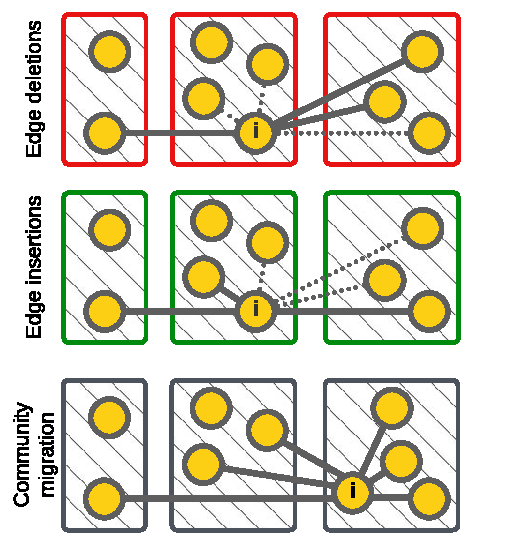
\includegraphics[width=0.3\linewidth]{out/about-cases-naive.pdf}
  }
  \subfigure{
    \label{fig:cases-delta-}
    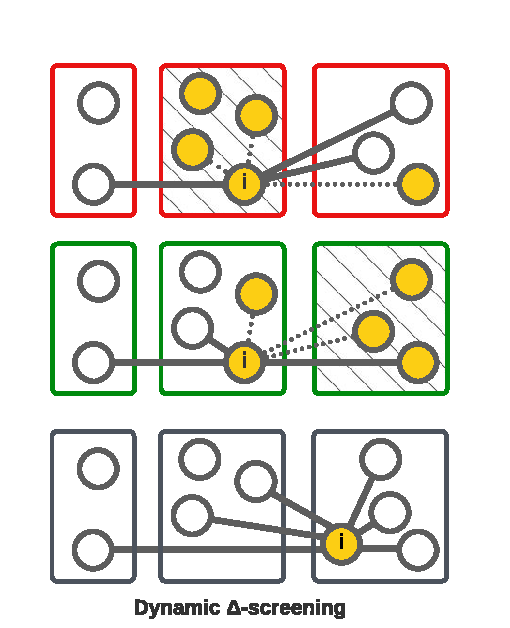
\includegraphics[width=0.3\linewidth]{out/about-cases-delta.pdf}
  }
  \subfigure{
    \label{fig:cases-frontier}
    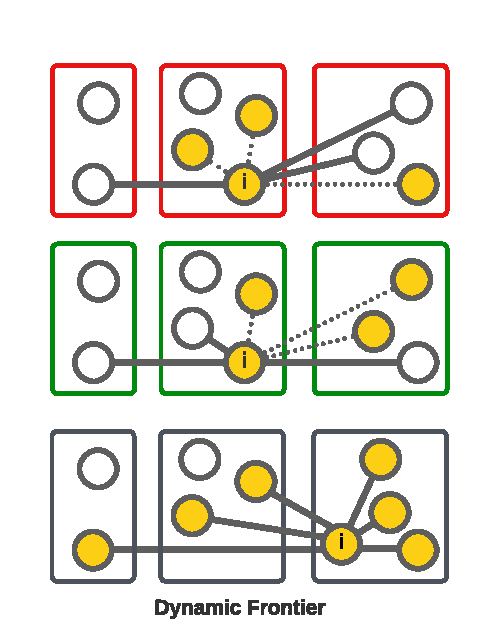
\includegraphics[width=0.3\linewidth]{out/about-cases-frontier.pdf}
  } \\[-2ex]
  \caption{Comparison of dynamic community detection approaches: \textit{Naive-dynamic} (\Nai{}), \textit{Dynamic $\Delta$-screening} (\Del{}), and \textit{Dynamic Frontier} (\Fro{}). Vertices marked as affected (initially) with each approach are highlighted in yellow, and when entire communities are marked as affected, they are hatched.}
  \label{fig:dynamic-approaches}
\end{figure*}

\begin{figure*}[!hbtp]
  \centering
  \subfigure[]{
    \label{fig:frontier-example-01}
    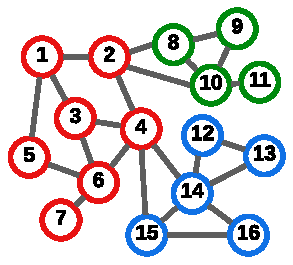
\includegraphics[width=0.18\linewidth]{out/about-frontier-01.pdf}
  }
  % \subfigure{
  %   \label{fig:frontier-example-02}
  %   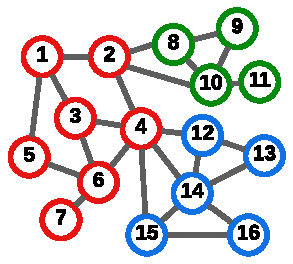
\includegraphics[width=0.15\linewidth]{out/about-frontier-02.pdf}
  % }
  \subfigure[]{
    \label{fig:frontier-example-03}
    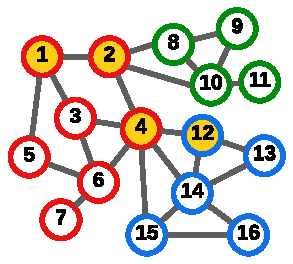
\includegraphics[width=0.18\linewidth]{out/about-frontier-03.pdf}
  }
  \subfigure[]{
    \label{fig:frontier-example-04}
    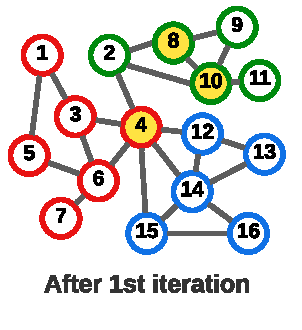
\includegraphics[width=0.18\linewidth]{out/about-frontier-04.pdf}
  }
  \subfigure[]{
    \label{fig:frontier-example-05}
    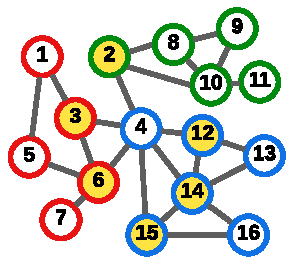
\includegraphics[width=0.18\linewidth]{out/about-frontier-05.pdf}
  }
  \subfigure[]{
    \label{fig:frontier-example-06}
    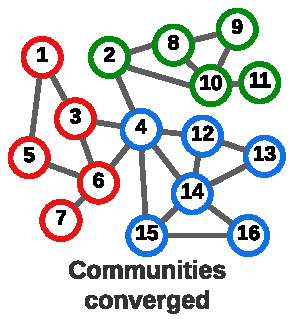
\includegraphics[width=0.18\linewidth]{out/about-frontier-06.pdf}
  } \\[-2ex]
  \caption{An example explaining the \textit{Dynamic Frontier} approach (\Fro{}). The community membership of each vertex is shown with border color (red, green, or blue), and the algorithm proceeds from left to right. A batch update arrives, affecting vertices $1$, $2$, $4$, and $12$. In the first iteration, vertex $2$ switches from red to green, impacting neighbors $8$ and $10$. In the second iteration, vertex $4$ changes from red to blue, affecting neighbors $3$, $6$, $12$, $14$, and $15$. Afterward, there are no more community changes.}
  % An example explaining the \textit{Dynamic Frontier} approach (\Fro{}). The community membership of each vertex is shown with border color (red, green, or blue), and the algorithm proceeds from left to right. \su{A batch update arrives, consisting of $\Delta^{t-}=\{(1, 2)\}$ and $\Delta^{t+}=\{(4, 12)\}$. Initially, \Fro{} marks vertices $1$, $2$, $4$, and $12$ as affected. In the first iteration, $2$ changes its membership from \textit{red} to \textit{green}, affecting neighbors $8$ and $10$. In the second iteration, $4$ changes its community from \textit{red} to \textit{blue}, affecting neighbors $3$, $6$, $12$, $14$, and $15$. Subsequently, no further community changes occur.
  \label{fig:frontier-example}
\end{figure*}


Given a batch update on the original graph, it is likely that only a small subset of vertices in the graph would change their community membership. Selection of the appropriate set of affected vertices to be processed (that are likely to change their community), in addition to the overhead of finding them, plays a significant role in the overall accuracy and efficiency of a dynamic batch parallel algorithm. Too small a subset may result in poor-quality communities, while a too-large subset will increase computation time. However, \Nai{} processes all the vertices, while \Del{} generally overestimates the set of affected vertices and has a high overhead. Our proposed \textit{Dynamic Frontier} approach (which we from here on refer to as \Fro{}) addresses these issues.


\subsubsection{Explanation of the approach}

We now explain \Fro{}. Consider a batch update consisting of edge deletions $(i, j) \in \Delta^{t-}$ and insertions $(i, j, w) \in \Delta^{t+}$, shown with double-dashed lines and double-solid lines respectively, with respect to a single source vertex $i$, in Figure \ref{fig:dynamic-approaches}. At the start of the community detection algorithm, we initialize the community membership of each vertex to that obtained in the previous snapshot of the graph.

\paragraph{Initial marking of affected vertices on edge deletion/insertion}

For edge deletions between vertices belonging to the same community and edge insertions between vertices belonging to different communities, we mark the source vertex $i$ as affected, as shown with vertices highlighted in yellow, in Figure \ref{fig:dynamic-approaches}. Note that batch updates are undirected, so we effectively mark both the endpoints $i$ and $j$. Edge deletions between vertices lying across communities and edge insertions for vertices lying within the same community are ignored (for reasons stated before).

\paragraph{Incremental marking of affected vertices on vertex migration to another community}

When a vertex $i$ changes its community during the community detection algorithm (shown with an arrow, with the direction indicating the migration of source vertex $i$ from its previous community to another new community), we mark all its neighbor vertices $j \in J_i$ as affected, as shown if Figure \ref{fig:dynamic-approaches} (highlighted in yellow), and mark $i$ as not affected. To minimize unnecessary computation, we also mark an affected vertex $i$ as not affected even if  $i$ does not change its community. We call this as the vertex pruning optimization. The process is akin to a graph traversal and continues until the communities have converged.

\paragraph{Application to the first pass of Louvain algorithm}

We apply \Fro{} to the first pass of \Lou{} algorithm (see Line \ref{alg:louvain--remark-pass} in Algorithm \ref{alg:louvain}), as with \Del{}. In subsequent passes, if the aggregation tolerance condition is not met (Line \ref{alg:louvain--aggregation-tolerance} in Algorithm \ref{alg:louvain}), all super-vertices are marked as affected and processed according to Louvain. This takes less than $14\%$ of total time, so we don't use \Fro{} to find affected super-vertices. The tolerance condition only fails in the case of large batch updates.


\subsubsection{A simple example}

Figure \ref{fig:frontier-example} shows an example of \Fro{}.

\paragraph{Initial communities}

The original graph comprises a total of $16$ vertices, which are divided into three communities, distinguished by the border colors of \textit{red}, \textit{green}, and \textit{blue} (see Figure \ref{fig:frontier-example-01}). This community membership information of each vertex could have been obtained by executing either the static or dynamic version of the \Lou{}/\LPA{} algorithm.

\paragraph{Batch update and Marking affected (initial)}

Subsequently a batch update is applied to the original graph (see Figure \ref{fig:frontier-example-03}), involving the deletion of an edge between vertices $1$ and $2$, and the insertion of an edge between vertices $4$ and $12$. Following the batch update, we perform the initial step of \Fro{}, marking endpoints $1$, $2$, $4$, and $12$ as affected. At this point, we are ready to execute the first iteration of a community detection algorithm.

\paragraph{After first iteration}

During the first iteration (see Figure \ref{fig:frontier-example-04}), the community membership of vertex $2$ changes from \textit{red} to \textit{green} because it exhibits stronger connections with vertices in the \textit{green} community. In response to this change, the \Fro{} incrementally marks the neighboring vertices of $2$ as affected, specifically vertices $8$ and $10$. Vertex $2$ is no longer marked as affected due to pruning.

\paragraph{After second iteration}

Let us now consider the second iteration (see Figure \ref{fig:frontier-example-05}). Vertex $4$ is now more strongly connected to the \textit{blue} community, resulting in a change of its community membership from \textit{red} to \textit{blue}. As before, we mark the neighbors of vertex $4$ as affected, namely vertices $12$, $14$, and $15$. Vertex $4$, once again, no longer marked as affected due to vertex pruning.

\paragraph{Communities converged}

In the subsequent iteration (see Figure \ref{fig:frontier-example-06}), no other vertices have a strong enough reason to change their community membership. At this point, when employing \Lou{}, the aggregation phase commences consolidating communities into super-vertices to prepare for the subsequent pass of the algorithm. However, when employing the \LPA{}, this marks the conclusion of the algorithm.

\begin{algorithm}[hbtp]
\caption{GVE-Louvain: Our parallel Louvain algorithm.}
\label{alg:louvain}
\begin{algorithmic}[1]
\Require{$G$: Input graph}
\Require{$C$: Community membership of each vertex}
\Require{$G'$: Input/super-vertex graph}
\Require{$C'$: Community membership of each vertex in $G'$}
\Require{$K'$: Total edge weight of each vertex}
\Require{$\Sigma'$: Total edge weight of each community}
\Ensure{$G'_{C'}$: Community vertices (CSR)}
\Ensure{$H_t$: Collision-free per-thread hashtable}
\Ensure{$l_i$: Number of iterations performed (per pass)}
\Ensure{$l_p$: Number of passes performed}
\Ensure{$\tau$: Per iteration tolerance}
\Ensure{$\tau_{agg}$: Aggregation tolerance}

\Statex

\Function{louvain}{$G$} \label{alg:louvain--begin}
  \State Vertex membership: $C \gets [0 .. |V|)$ \textbf{;} $G' \gets G$ \label{alg:louvain--initialization}
  \ForAll{$l_p \in [0 .. \text{\small{MAX\_PASSES}})$} \label{alg:louvain--passes-begin}
    \State $\Sigma' \gets K' \gets vertexWeights(G')$ \textbf{;} $C' \gets [0 .. |V'|)$ \label{alg:louvain--reset-weights}
    \State Mark all vertices in $G'$ as unprocessed \label{alg:louvain--reset-affected}
    \State $l_i \gets louvainMove(G', C', K', \Sigma')$ \label{alg:louvain--local-move}
    \If{$l_i \le 1$} \textbf{break} \Comment{Globally converged?} \label{alg:louvain--globally-converged}
    \EndIf
    \State $|\Gamma|, |\Gamma_{old}| \gets$ Number of communities in $C$, $C'$
    \If{$|\Gamma|/|\Gamma_{old}| > \tau_{agg}$} \textbf{break} \Comment{Low shrink?} \label{alg:louvain--aggregation-tolerance}
    \EndIf
    \State $C' \gets$ Renumber communities in $C'$ \label{alg:louvain--renumber}
    \State $C \gets$ Lookup dendrogram using $C$ to $C'$ \label{alg:louvain--lookup}
    \State $G' \gets louvainAggregate(G', C')$ \label{alg:louvain--aggregate}
    \State $\tau \gets \tau / \text{\small{TOLERANCE\_DROP}}$ \Comment{Threshold scaling} \label{alg:louvain--threshold-scaling}
  \EndFor \label{alg:louvain--passes-end}
  \State $C \gets$ Lookup dendrogram using $C$ to $C'$ \label{alg:louvain--lookup-last}
  \Return{$C$} \label{alg:louvain--return}
\EndFunction \label{alg:louvain--end}
\end{algorithmic}
\end{algorithm}

\begin{figure}[hbtp]
  \centering
  \subfigure{
    \label{fig:adjust-auxiliary--8020}
    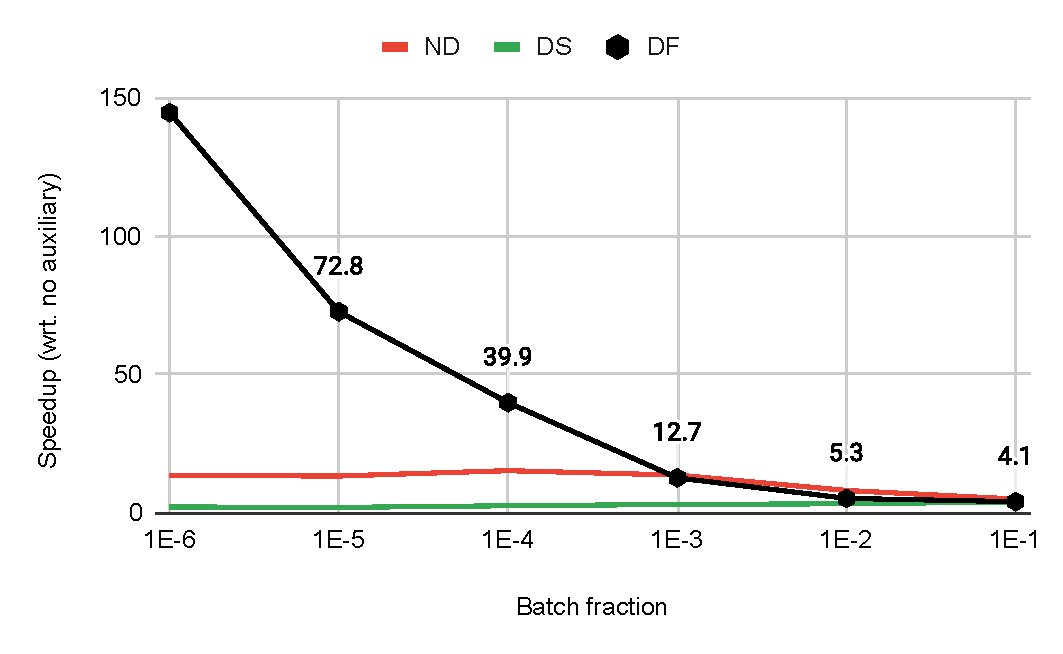
\includegraphics[width=0.98\linewidth]{out/adjust-auxiliary-8020.pdf}
  } \\[-2ex]
  \caption{Speedup of \textit{Naive-dynamic (ND)}, \textit{Delta-screening (DS)}, and \textit{Dynamic Frontier (DF)} Louvain when reusing the previous \textit{weighted-degrees of vertices} and \textit{total edge weight of communities} as auxiliary information to the dynamic algorithm, compared to the same dynamic algorithm when both are recomputed from scratch. This is done on large graphs with generated random batch updates of size $10^{-7} |E|$ to $0.1 |E|$\ignore{, consisting of $80\%$ edge insertions and $20\%$ deletions, to simulate realistic dynamic graph updates}.}
  \label{fig:adjust-auxiliary}
\end{figure}





\subsection{Our Dynamic Frontier based Louvain (\FroLou{}, Algorithm \ref{alg:louvain})}
\label{sec:dynamic-louvain}

We show how to apply our \textit{Dynamic Frontier} approach (\Fro{}) to \Lou{} in Algorithm \ref{alg:louvain} (which we call \FroLou{}). We take as input the previous snapshot of the graph $G^{t-1}$, the previous community membership of each vertex $C^{t-1}$, and the batch update consisting of edge deletions $\Delta^{t-}$ and insertions $\Delta^{t+}$ in Line \ref{alg:louvain--main-begin}. First, in Lines \ref{alg:louvain--restart-begin}-\ref{alg:louvain--restart-end}, we check if we should use \StaLou{} to maintain the quality of communities (explained in Section \ref{sec:restart}). Then, in Lines \ref{alg:louvain--mark-begin}-\ref{alg:louvain--mark-end}, based on \Fro{}, we mark the initial set of vertices as affected. In Lines \ref{alg:louvain--membership} and \ref{alg:louvain--super-membership-begin}-\ref{alg:louvain--super-membership-end}, we initialize the community membership of each vertex in the graph $G^t$, and each super-vertex in the aggregated graph $G'$ (in the first pass, this is the same as the input graph $G^t$).

For each pass (Lines \ref{alg:louvain--passes-begin}-\ref{alg:louvain--passes-end}), we perform the \textit{local-moving} phase of \Lou{} in Line \ref{alg:louvain--local-move}. If the community labels converge after one iteration, we terminate the algorithm (Line \ref{alg:louvain--globally-converged}). In Line \ref{alg:louvain--renumber}, we renumber the community-ids. This renumbering helps generate the aggregated graph $G'$ in the Compressed Sparse Row (CSR) format and counting the number of communities. In Line \ref{alg:louvain--lookup}, we update the community membership of each vertex $C$ based on the community membership of each super-vertex, such that we refer to the top-level hierarchy of the dendrogram as the final result.

Next, at Line \ref{alg:louvain--aggregation-tolerance}, we check whether only a small portion of communities have merged together. To do this, we calculate the ratio of the number of communities after the \textit{local-moving} phase $|\Gamma|$ to the original number of communities $|\Gamma_{old}|$. If this ratio $|\Gamma|/|\Gamma_{old}|$ is less than a specific value called the aggregation tolerance ($\tau_{agg}$, whose optimal value is measured and mentioned in Section \ref{sec:louvain}), it means that the merging has been minimal. In such a situation, we stop the algorithm to avoid the computationally expensive \textit{aggregation} phase, as it doesn't provide significant benefits. However, if a sufficiently large number of communities have merged together, we proceed with the \textit{aggregation} phase and obtain the aggregated graph $G'$. This graph is stored in CSR format.

Next, we perform the threshold scaling optimization \cite{com-naim17}, i.e., we reduce the tolerance $\tau$ by a tolerance drop factor of \verb|TOLERANCE_DROP|. This optimization helps minimize the number of iterations performed in the local-moving phase of \Lou{}. It improves performance with little sacrifice in the quality of communities obtained.

We now discuss the \textit{local-moving} phase of \Lou{}. First, in Lines \ref{alg:louvain--edge-weigths-begin}-\ref{alg:louvain--edge-weigths-end}, we calculate the total edge weights linked to each vertex $K'$ and the total edge weights linked to each community $\Sigma'$. For each iteration (Lines \ref{alg:louvain--iterations-begin}-\ref{alg:louvain--iterations-end}), and for each affected vertex $i$ in the graph $G'$, we use per-thread collision-free hashtables to obtain the best community linked to each vertex $c^*$, as well as the associated delta-modularity (highest) $\delta Q^*$ in parallel using Equation \ref{eq:delta-modularity} (Lines \ref{alg:louvain--best-community-begin}-\ref{alg:louvain--best-community-end}). If the best community $c^*$ is different from the original community membership $C'[i]$ of vertex $i$ (Line \ref{alg:louvain--best-community-same}), we update the community membership of the vertex and atomically update the total edge weights linked to each community in Lines \ref{alg:louvain--perform-move-begin}-\ref{alg:louvain--perform-move-end}. In addition, if this is the first pass of \Lou{} (Line \ref{alg:louvain--remark-pass}), based on \Fro{}, we mark the neighbors of vertex $i$ as affected in Line \ref{alg:louvain--remark}. To minimize unnecessary computation, we also mark vertex $i$ as not affected (whether or not $i$ changes its community) as part of vertex pruning optimization in Line \ref{alg:louvain--prune}. At the end of each iteration, if the total delta-modularity across all vertices $\Delta Q$ is less than the specified tolerance $\tau$, we terminate the local-moving phase (Line \ref{alg:louvain--locally-converged}). We prove the correctness of \FroLou{} in Section \ref{sec:louvain-correctness}.




\subsection{Maintaining quality across batches}
\label{sec:restart}

In our experiments with continuous batch updates of edge insertions of size $10^{-3} |E|$, we find that the quality of communities obtained using the \DelLou{} and \FroLou{} starts to drop (compared to \StaLou{}) by $48\%$ (rapid decline) and $5.7\%$ respectively after around $1300$ batches of updates. The same happens for \FroHyb{} by $10\%$ after around $600$ updates. Therefore, we conservatively use a \verb|RESTART_LOUVAIN| of $1000$, and a \verb|RESTART_HYBRID| of $500$ (see Lines \ref{alg:louvain--restart-begin}-\ref{alg:louvain--restart-end} in Algorithm \ref{alg:louvain}, and Lines \ref{alg:hybrid--restart-begin}-\ref{alg:hybrid--restart-end} in Algorithm \ref{alg:hybrid}). As the lines show, we run \StaLou{} once for $1000$/$500$ batches of updates to maintain the quality of communities across multiple batch updates and correct the error introduced. We adjust our reported timings by amortizing its cost.




\subsection{Time and Space complexity}
\label{sec:complexity}

To analyze the time complexity of our algorithms, we use $N_B$ to denote the number of vertices marked as affected (which is dependent on the size and nature of batch update) by the dynamic algorithm on a batch $B$ of edge updates, use $M_B$ to denote the number of edges with one endpoint in $N_B$, and $K$ to denote the total number of iterations performed. Then the time complexity of Algorithms \ref{alg:louvain}-\ref{alg:hybrid} is $O(K M_B)$. In the worst case, the time complexity of our algorithms would be the same as that of the respective static algorithms, i.e., $O(KM)$. The space complexity of our algorithms is the same as that of the static algorithms, i.e., $O(N + M)$.


\section{Evaluation}
\label{sec:evaluation}
\subsection{Experimental setup}
\label{sec:setup}

\subsubsection{System}
\label{sec:system}

For our experiments, we use a server that has an x86-based 64-bit AMD EPYC-7742 processor. This processor has a clock frequency of 2.25 GHz and 512 GB of DDR4 system memory. Each core has an L1 cache of 4 MB, an L2 cache of 32 MB, and a shared L3 cache of 256 MB. The machine runs on Ubuntu 20.04. We use GCC 9.4 and OpenMP 5.0 \cite{openmp18}.


\subsubsection{Configuration}
\label{sec:configuration}

We use 32-bit unsigned integer for vertex ids, 32-bit floating point for edge weights, but use 64-bit floating point for hashtable values, total edge weight, modularity calculation, and all places where performing an aggregation/sum of floating point values. Unless mentioned otherwise, we execute all parallel implementations with a default of $64$ threads (to match the number of cores available on the system).

\begin{table}[hbtp]
  \centering
  \caption{List of $13$ graphs obtained SuiteSparse Matrix Collection \cite{suite19} (directed graphs are marked with $*$). Here, $|V|$ is the number of vertices, $|E|$ is the number of edges (after adding reverse edges), $D_{avg}$ is the average degree, and $|\Gamma|$ is the number of communities obtained using Louvain algorithm.\ignore{In the table, B refers to a billion, M refers to a million and K refers a thousand.}}
  \label{tab:dataset}
  \begin{tabular}{|c||c|c|c|c|}
    \toprule
    \textbf{Graph} &
    \textbf{\textbf{$|V|$}} &
    \textbf{\textbf{$|E|$}} &
    \textbf{\textbf{$D_{avg}$}} &
    \textbf{\textbf{$|\Gamma|$}} \\
    % \textbf{$1 - \Gamma_G$} \\
    \midrule
    \multicolumn{5}{|c|}{\textbf{Web Graphs (LAW)}} \\ \hline
    indochina-2004$^*$ & 7.41M & 341M & 41.0 & 4.24K \\ \hline  % & \num{4.7e-4} & 2.9 GB
    uk-2002$^*$ & 18.5M & 567M & 16.1 & 42.8K \\ \hline  % & \num{9.6e-5} & 16 GB
    arabic-2005$^*$ & 22.7M & 1.21B & 28.2 & 3.66K \\ \hline  % & \num{5.5e-4} & 11 GB
    uk-2005$^*$ & 39.5M & 1.73B & 23.7 & 20.8K \\ \hline  % & \num{9.6e-5} & 16 GB
    webbase-2001$^*$ & 118M & 1.89B & 8.6 & 2.76M \\ \hline  % & \num{7.3e-7} & 18 GB
    it-2004$^*$ & 41.3M & 2.19B & 27.9 & 5.28K \\ \hline  % & \num{3.8e-4} & 19 GB
    sk-2005$^*$ & 50.6M & 3.80B & 38.5 & 3.47K \\ \hline  % & \num{5.8e-4} & 33 GB
    \multicolumn{5}{|c|}{\textbf{Social Networks (SNAP)}} \\ \hline
    com-LiveJournal & 4.00M & 69.4M & 17.4 & 2.54K \\ \hline  % & \num{7.9e-4} & 480 MB
    com-Orkut & 3.07M & 234M & 76.2 & 29 \\ \hline  % & \num{6.7e-2} & 1.7 GB
    \multicolumn{5}{|c|}{\textbf{Road Networks (DIMACS10)}} \\ \hline
    asia\_osm & 12.0M & 25.4M & 2.1 & 2.38K \\ \hline  % & \num{8.4e-4} & 200 MB
    europe\_osm & 50.9M & 108M & 2.1 & 3.05K \\ \hline  % & \num{6.6e-4} & 910 MB
    \multicolumn{5}{|c|}{\textbf{Protein k-mer Graphs (GenBank)}} \\ \hline
    kmer\_A2a & 171M & 361M & 2.1 & 21.2K \\ \hline  % & \num{9.4e-5} & 3.2 GB
    kmer\_V1r & 214M & 465M & 2.2 & 6.17K \\ \hline  % & \num{3.2e-4} & 4.2 GB
  \bottomrule
  \end{tabular}
\end{table}
% We convert directed graphs (marked with $*$) to undirected by duplicating edges in the reverse direction, and set the weight of each edge to $1$. and $F_{size}$ is size of the \textit{MatrixMarket} file



\subsubsection{Reproducibility}
\label{sec:reproducibilty}

All our results are reproducible. The source code for the experiments reported in this paper along with necessary scripts for obtaining the datasets and compiling the software is available at \url{https://bit.ly/hipc23-174}. 


\subsubsection{Dataset}
\label{sec:dataset}

Table \ref{tab:dataset} shows the graphs we use in our experiments. All of them are obtained from the SuiteSparse Matrix Collection \cite{suite19}. The number of vertices in the graphs varies from $3.07$ to $214$ million, and the number of edges varies from $25.4$ million to $3.80$ billion. We ensure that all edges are undirected and weighted with a default weight of $1$.


\subsubsection{Batch generation}
\label{sec:batch-update}

We take a base graph from the dataset and generate a random batch update \cite{com-zarayeneh21} consisting of an equal mix of edge deletions and insertions \cite{com-chong13}, each with an edge weight of $1$. All batch updates are undirected, i.e., for every edge insertion $(i, j, w)$ in the batch update, the edge $(j, i, w)$ is also a part of the batch update. For simplicity, we generate these edges such that the selection of each vertex (as endpoint) is equally probable, and we do not add any new vertices to the graph. Testing with batches having other distributions is part of our future work.

\begin{figure*}[hbtp]
  \centering
  \subfigure[Results of each graph]{
    \label{fig:louvain--all}
    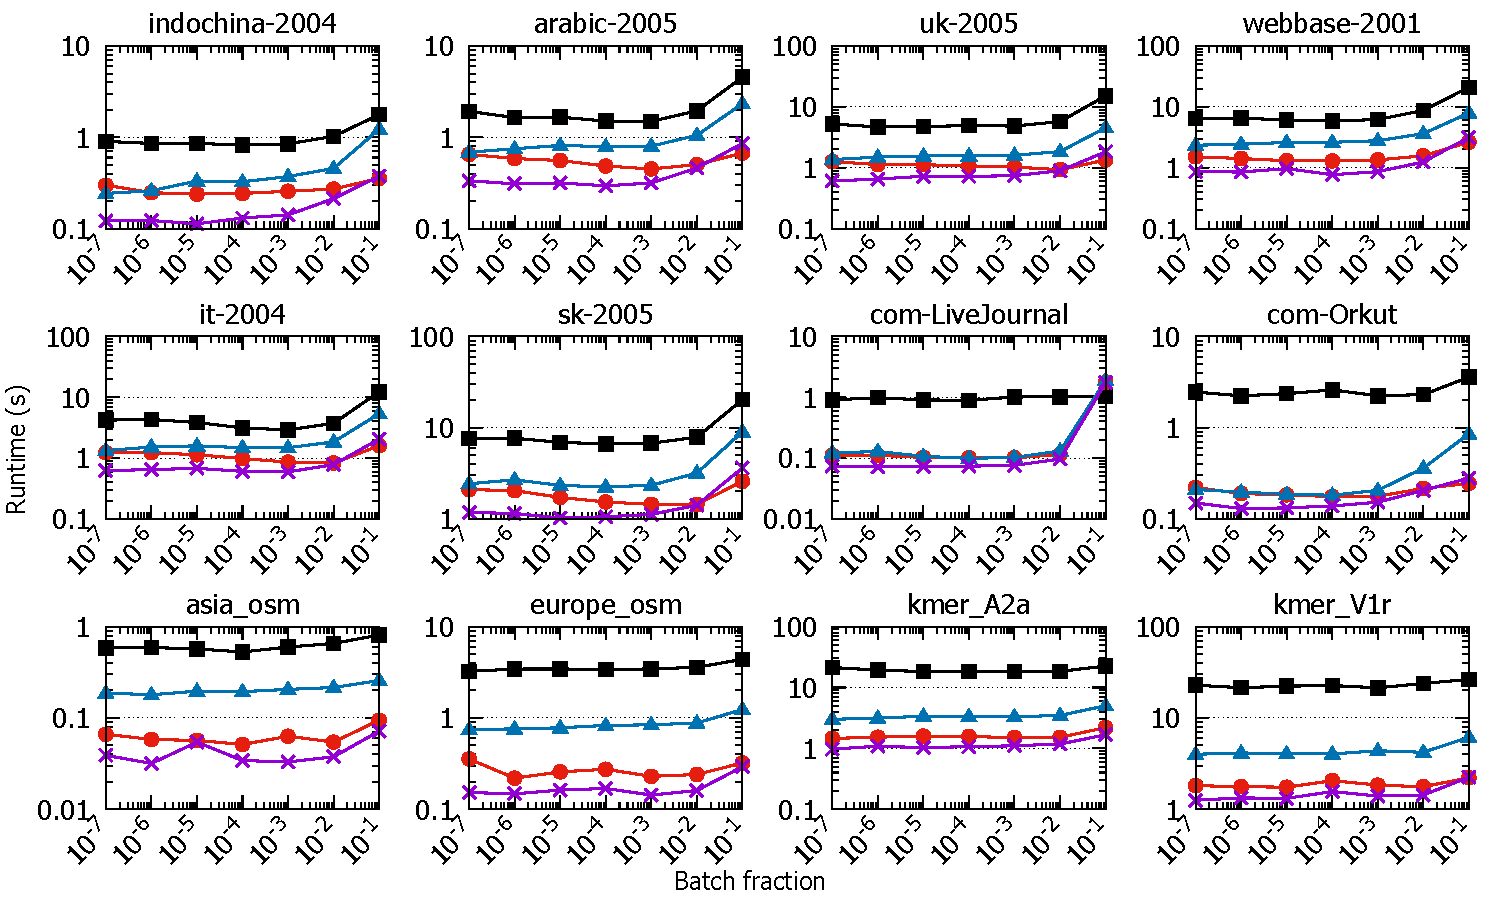
\includegraphics[width=0.58\linewidth]{out/louvain-all-fullx.pdf}
  }
  \subfigure[Overall result]{
    \label{fig:louvain--am}
    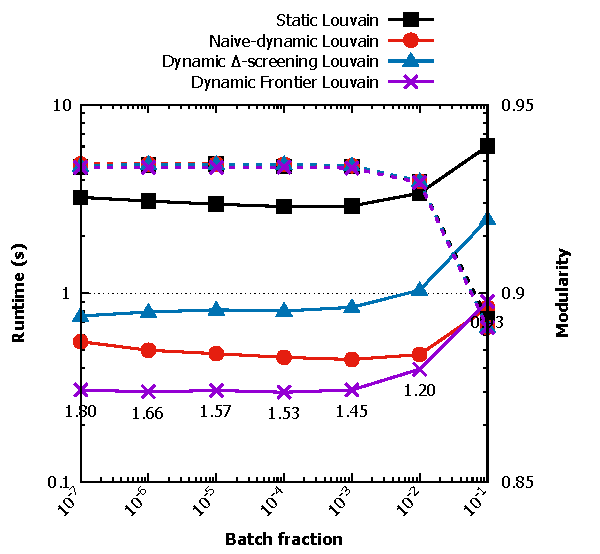
\includegraphics[width=0.38\linewidth]{out/louvain-am.pdf}
  } \\[-2ex]
  \caption{Time taken (solid lines), and modularity of communities obtained (dashed lines) along the right Y-axis, with \StaLou{}, \NaiLou{}, \DelLou{}, and \FroLou (Algorithm \ref{alg:louvain}) on batch updates of increasing size from $10^{-7} |E|$ to $0.1 |E|$. Note that both axes are logarithmic. Speedup of \FroLou{} with respect to \NaiLou{} is labeled.}
  \label{fig:louvain}
\end{figure*}

\begin{figure*}[hbtp]
  \centering
  \subfigure[Results of each graph]{
    \label{fig:rak--all}
    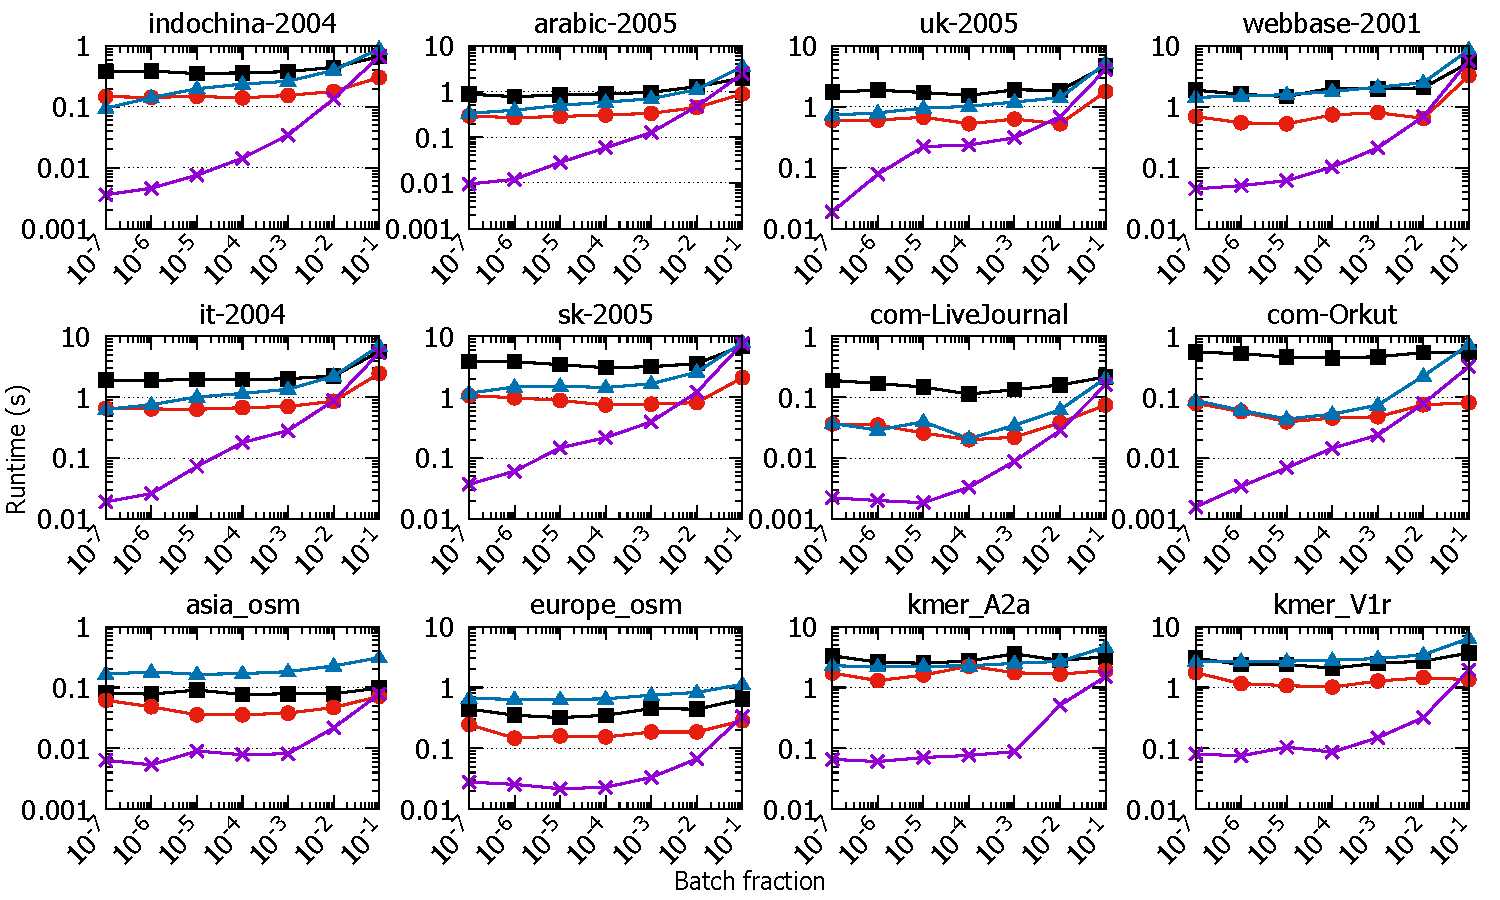
\includegraphics[width=0.58\linewidth]{out/rak-all-fullx.pdf}
  }
  \subfigure[Overall result]{
    \label{fig:rak--am}
    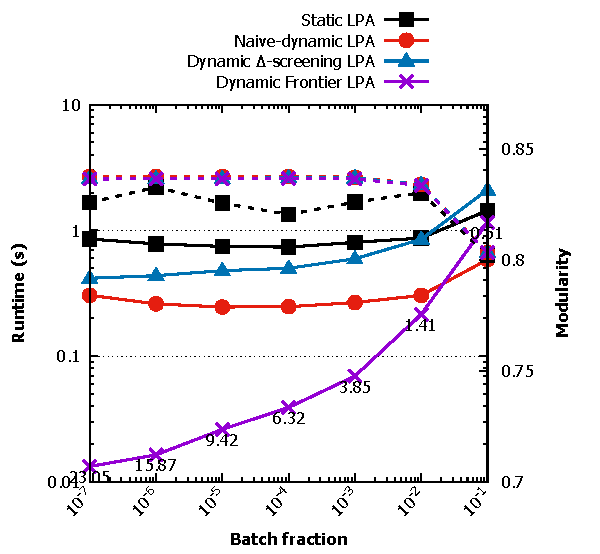
\includegraphics[width=0.38\linewidth]{out/rak-am.pdf}
  } \\[-2ex]
  \caption{Time taken (solid lines), and modularity of communities obtained (dashed lines) along the right Y-axis, with \StaLPA{}, \NaiLPA{}, \DelLPA{}, and \FroLPA{} (Algorithm \ref{alg:rak}) on batch updates of increasing size from $10^{-7} |E|$ to $0.1 |E|$. Note that both axes are logarithmic. Speedup of \FroLPA{} with respect to \NaiLPA{} is labeled.}
  \label{fig:rak}
\end{figure*}


\paragraph{Adjusting batch size}

For all dynamic graph-based experiments, we modify the batch size as a fraction of the total number of edges in the original (undirected) graph from $10^{-7}$ to $0.1$ (i.e., $10^{-7}|E|$ to $0.1|E|$). For a billion-edge graph, this amounts to a batch size of $100$ to $100$ million edges. Keep in mind that dynamic graph algorithms are helpful for small batch sizes in interactive applications. For large batches, it is usually more efficient to run the static algorithm.

\paragraph{Minimizing measurement noise}

We employ $5$ distinct random batch updates for each batch size and report average across these runs in our experiments.


\subsubsection{Determining optimality of result}
\label{sec:evaluation--optimality}

Community detection is an NP-hard problem and existing polynomial algorithms are \textit{heuristic}. We study correctness in terms of \textit{modularity score} of communities identified (higher is better), similar to previous works in the area \cite{com-traag19, com-zarayeneh21}. As Figures \ref{fig:louvain}-\ref{fig:hybrid} show, modularity of communities detected by our proposed dynamic algorithms is close to the modularity of communities detected by corresponding static algorithms.

\begin{figure*}[hbtp]
  \centering
  \subfigure[Dynamic Louvain algorithms]{
    \label{fig:louvainrak-affected--louvain}
    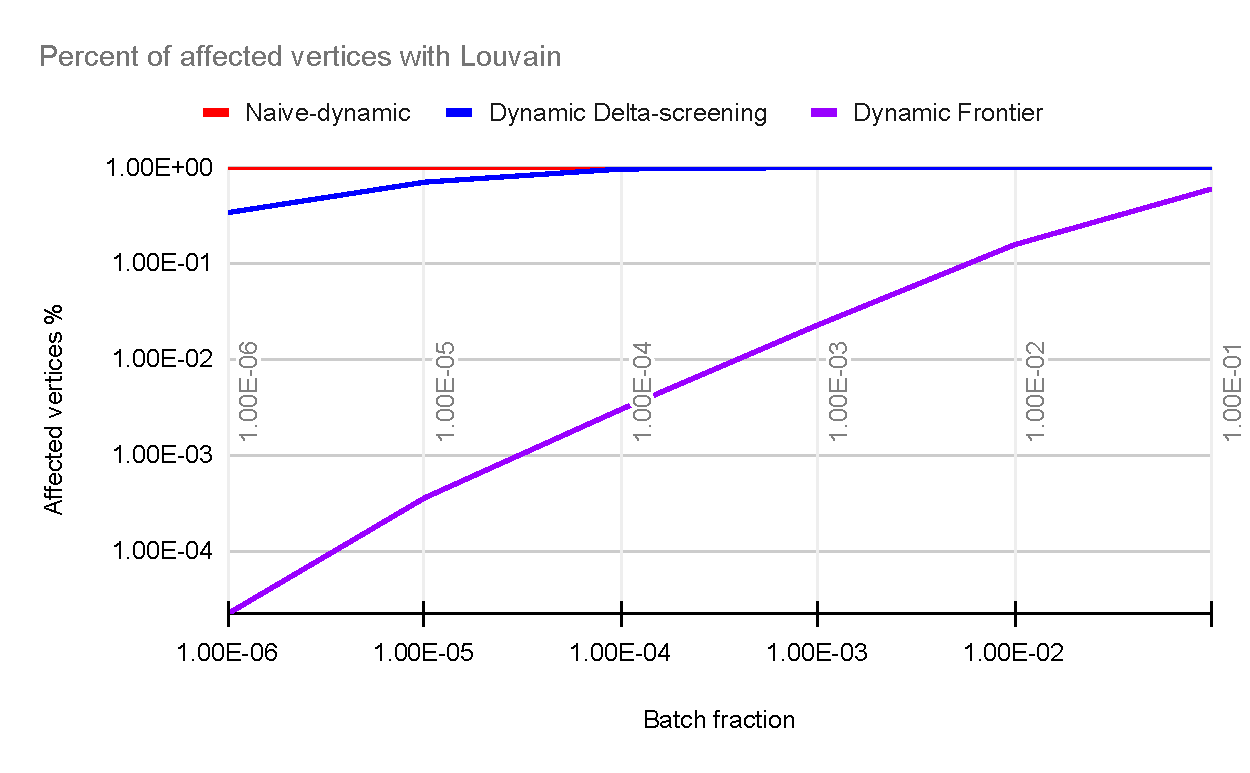
\includegraphics[width=0.48\linewidth]{out/louvain-affected.pdf}
  }
  \subfigure[Dynamic LPA algorithms]{
    \label{fig:louvainrak-affected--rak}
    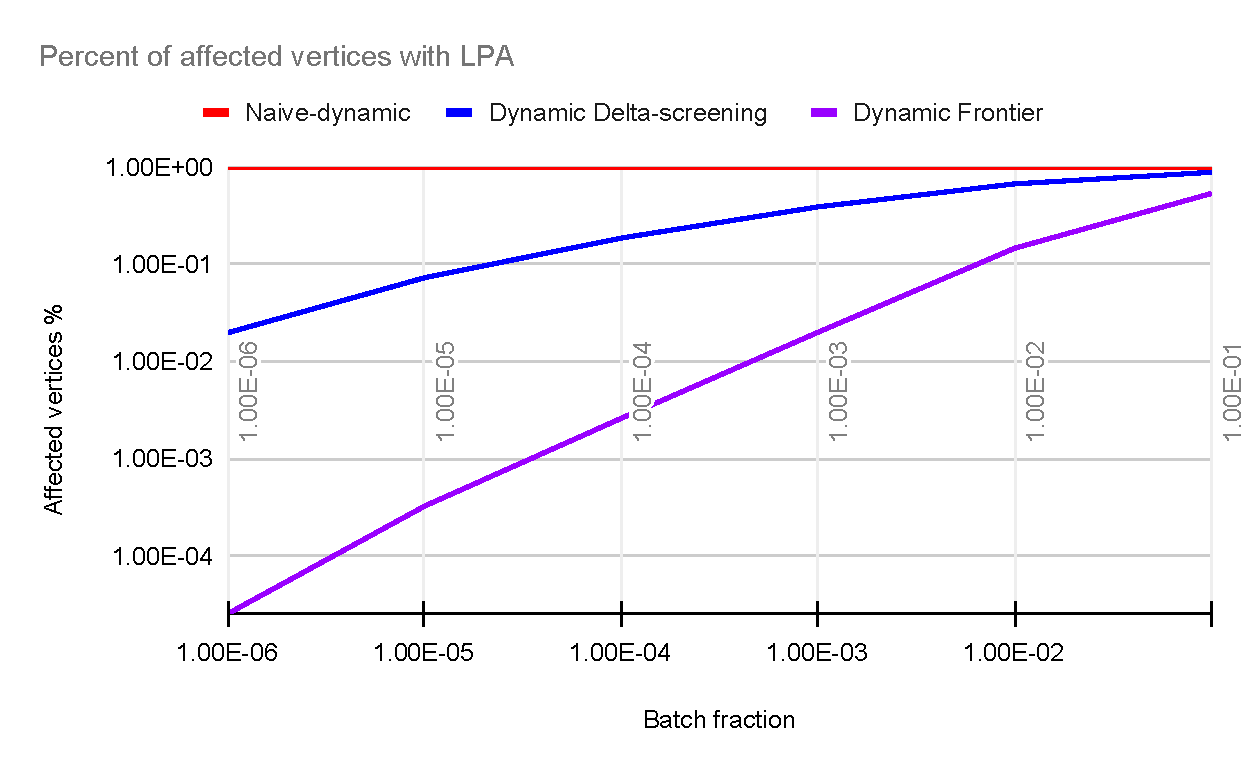
\includegraphics[width=0.48\linewidth]{out/rak-affected.pdf}
  } \\[-2ex]
  \caption{Percent of vertices marked as affected (mean) with \Nai{}, \Del{}, and \Fro{} based \Lou{} and \LPA{}, as mentioned in Sections \ref{sec:louvain-evaluation} and \ref{sec:rak-evaluation}, on graphs in Table \ref{tab:dataset}.}
  \label{fig:louvainrak-affected}
\end{figure*}

\begin{figure*}[hbtp]
  \centering
  \subfigure[Dynamic Louvain algorithms]{
    \label{fig:louvainrak-stability--louvain}
    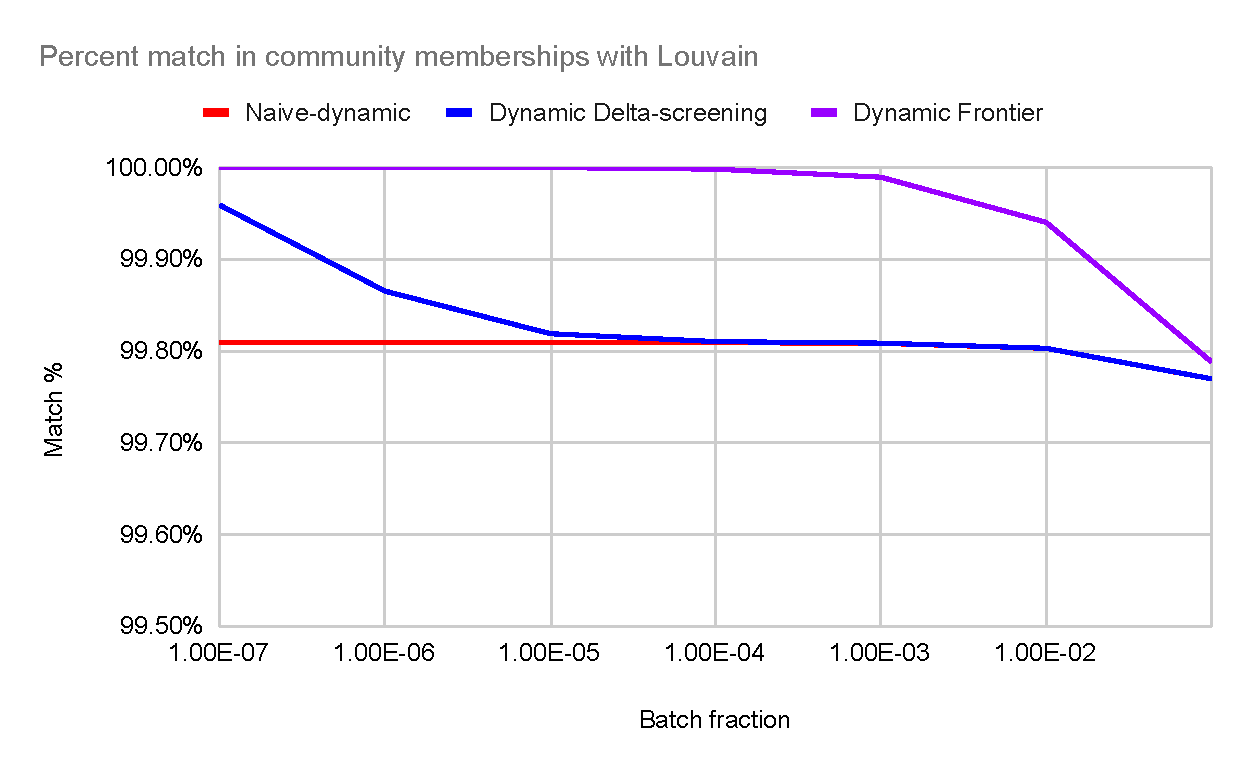
\includegraphics[width=0.48\linewidth]{out/louvain-stability.pdf}
  }
  \subfigure[Dynamic LPA algorithms]{
    \label{fig:louvainrak-stability--rak}
    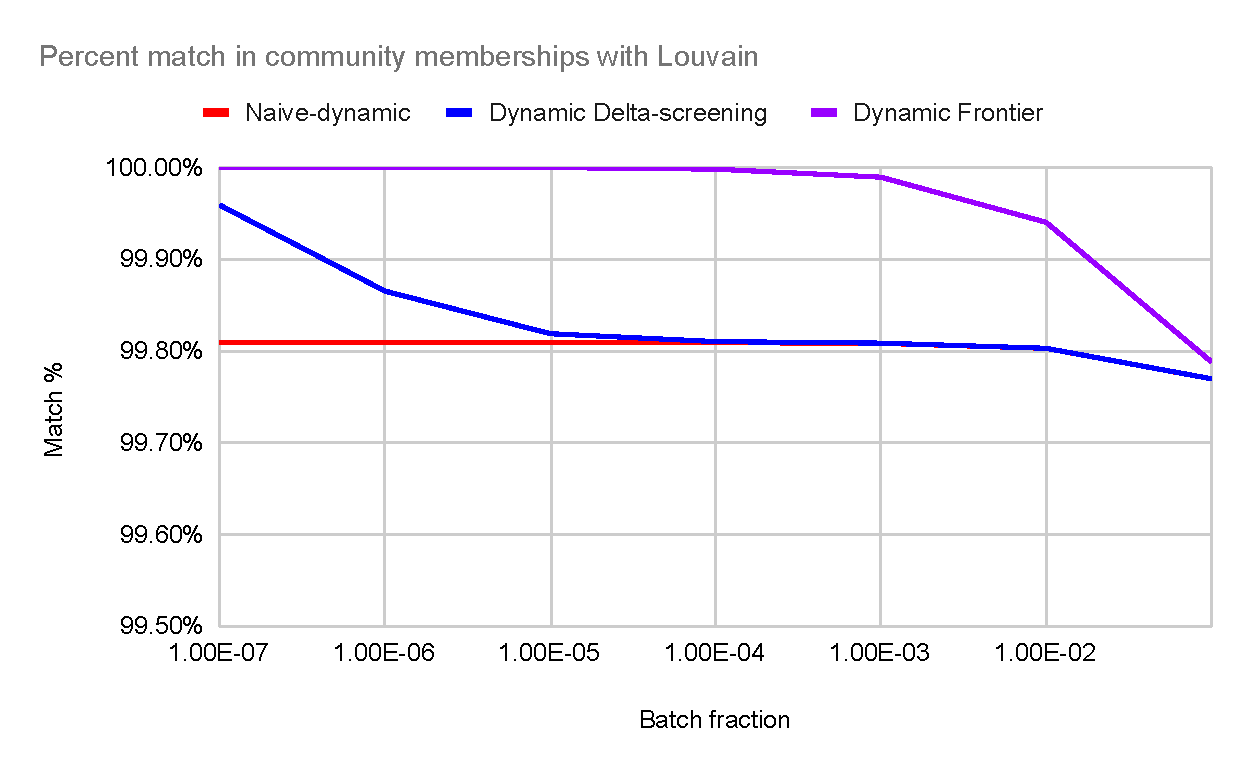
\includegraphics[width=0.48\linewidth]{out/louvain-stability.pdf}
  } \\[-2ex]
  \caption{Percent match in community memberships after reverse and forward batch updates (mean) with \Nai{}, \Del{}, and \Fro{} based \Lou{} and \LPA{}, as mentioned in Sections \ref{sec:louvain-stability} and \ref{sec:rak-stability}, on graphs in Table \ref{tab:dataset}.}
  \label{fig:louvainrak-stability}
\end{figure*}





\subsection{Performance of Dynamic Frontier Louvain (\FroLou{}, Algorithm \ref{alg:louvain})}
\label{sec:louvain-evaluation}

\subsubsection{Overall Performance}

We first study the performance of \FroLou{} on batch updates of size $10^{-7} |E|$ to $0.1 |E|$, and compare it with \StaLou{}, \NaiLou{}, and \DelLou{}. The work of Zarayeneh et al. \cite{com-zarayeneh21} demonstrates improved performance of \textit{$\Delta$-screening} compared to \textit{Dynamo} \cite{com-zhuang19} and \textit{Batch} \cite{com-chong13}. Thus, we limit our comparison to \Del{}. When executing \FroLou{} and \DelLou{}, we reinitialize the community memberships every \verb|RESTART_LOUVAIN| batches with the community labels obtained via \StaLou{} (see Section \ref{sec:restart}). As mentioned in Section \ref{sec:batch-update}, we generate $5$ different random batch updates for each batch size to minimize measurement noise.

Figure \ref{fig:louvain--am} shows the average results of the experiment. We observe the following from Figure \ref{fig:louvain--am}. The modularity of communities obtained by all the dynamic approaches is nearly identical. \FroLou{} converges the fastest with an average speedup of $1.5\times$ over \NaiLou{}. On small batch updates, atomics hinder the speedup. This isn't a reflection of our approach's inefficiency but rather a challenge posed by the parallel implementation of Louvain algorithm. As the batch size increases, the number of vertices marked as affected by \FroLou{} increases. This results in an increase in the time taken by \FroLou{} as the batch size increases. Further, as Figure \ref{fig:louvain--all} shows, dynamic approaches significantly outperform \StaLou{} on \textit{social networks}, \textit{road networks}, and \textit{k-mer protein graphs} (which do not have a dense community structure, or have a low $|E|/|V|$ ratio).

\paragraph{Performance of Dynamic $\Delta$-screening (\DelLou{})}

We note that \DelLou{} does not perform better than \NaiLou{}. This is because it tends to mark a large fraction of the vertices as affected, even for small batch updates. Our experiments on the graphs in Table \ref{tab:dataset} indicate that compared to the \FroLou{}, the \DelLou{} marks nearly $44\times$ more vertices as affected on a batch size of $10^{-3} |E|$.

\paragraph{Slowdown of static algorithm}

Uniform batches of insertions/deletions arbitrarily disrupt the original community structure. This results in \StaLou{} needing more iterations to converge.


\subsubsection{Comparison with respect to Riedy and Bader \cite{com-riedy13}}

Riedy and Bader propose a batch parallel dynamic algorithm for community detection. They compare the run time of their dynamic algorithm to that of a static recomputation. On the graphs \verb|caidaRouterLevel|, \verb|coPapersDBLP|, and \verb|eu-2005|, from \cite{com-riedy13} and at the batch size of $0.1|E|, 0.03|E|,$ and $0.1|E|$ respectively, they report a speedup of $40\times$, $1.08\times$, and $327\times$, respectively, over their corresponding static algorithm performing a full recomputation. On these three graphs and batch sizes, \FroLou{} achieves a speedup of $6.1\times$, $10.9\times$, and $4.2\times$, respectively, compared to a full static recomputation. This might compare unfavorably with the speedups claimed by Riedy and Bader \cite{com-riedy13}. However, note from Section \ref{sec:introduction} that the algorithm of Riedy and Bader \cite{com-riedy13} does not identify cascading changes to communities. In addition, as their source code is not available, we could not do a more direct comparison.


\subsubsection{Stability}
\label{sec:louvain-stability}

Intuitively, if the graphs $G^t$ and $G^{t'}$ are identical for some $t$ and $t'$, we expect \FroLou{} to produce the same communities for $G^t$ and $G^{t'}$. We refer to this property of a dynamic algorithm as its stability, measured as the percentage of vertices that agree on the community label across two identical graphs. Vertices within weak community structures tend to be unstable, as they may connect to multiple communities with similar strength.

To measure the stability of \NaiLou{}, \DelLou{}, and \FroLou{}, we proceed as follows. Let $G$ be an initial graph. We generate random batch updates of size $10^{-7} |E|$ to $0.1 |E|$ consisting of edge deletions to obtain the graph $G^1$. We then apply each of the above algorithms on $G^1$ to identify the new communities. Subsequently, we create another batch of updates that consists of inserting the edges deleted in the prior time step. This graph, $G^2$, is essentially the original graph $G$. We obtain the community labels of the vertices in the graph $G^2$ by appealing to the dynamic algorithms. Finally, we compare the community label of each vertex in the graphs $G$ and $G^2$. The resulting match in community membership of vertices with \NaiLou{}, \DelLou{}, and \FroLou{} on batch updates of size $10^{-7} |E|$ to $0.1 |E|$ is shown in Figure \ref{fig:louvainrak-stability--louvain}.

From Figure \ref{fig:louvainrak-stability--louvain}, we observe that\NaiLou{} and \DelLou{} have minimum of $99.68\%$ match with the original community memberships across all batch sizes, while \FroLou{} has a minimum of $99.70\%$ match. This indicates that all these algorithms are stable.

\begin{figure*}[hbtp]
  \centering
  \subfigure[Results of each graph]{
    \label{fig:hybrid--all}
    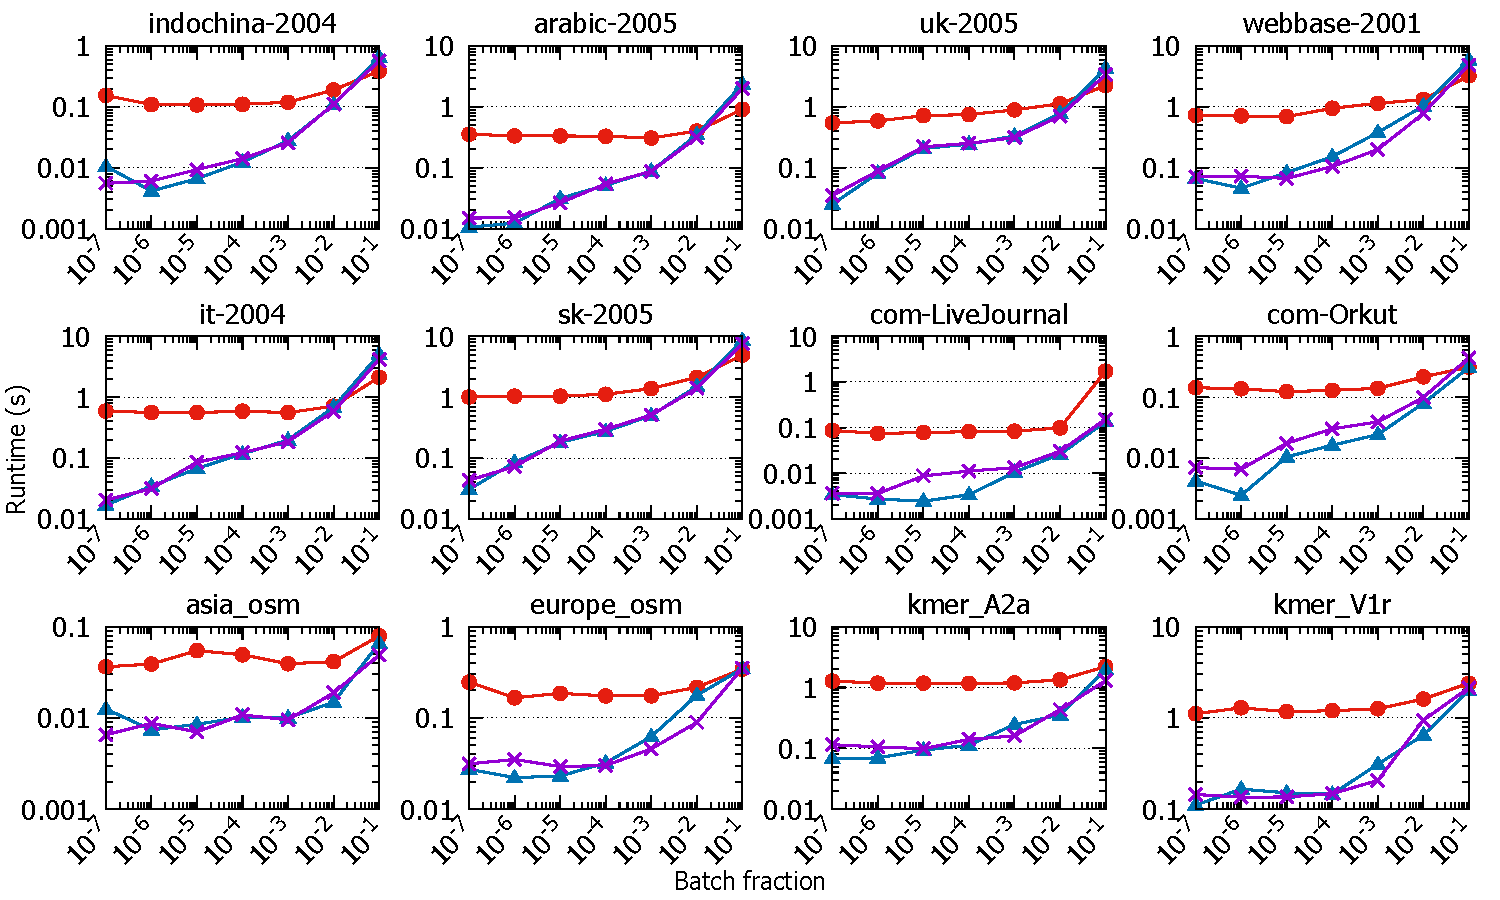
\includegraphics[width=0.58\linewidth]{out/hybrid-all-fullx.pdf}
  }
  \subfigure[Overall result]{
    \label{fig:hybrid--am}
    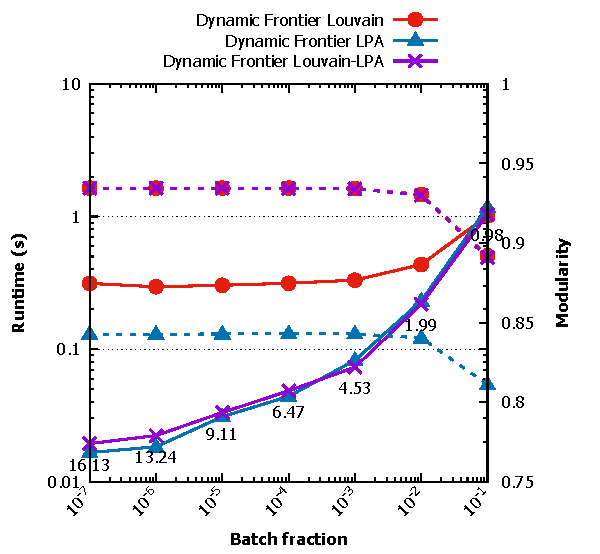
\includegraphics[width=0.38\linewidth]{out/hybrid-am.pdf}
  } \\[-2ex]
  \caption{Time taken (solid lines), and modularity of communities obtained (dashed lines) along the right Y-axis, with \FroLou{}, \FroLPA{}, and \FroHyb{} (Algorithms \ref{alg:louvain}, \ref{alg:rak}, and \ref{alg:hybrid}) on batch updates of increasing size from $10^{-7} |E|$ to $0.1 |E|$. Note that both axes are logarithmic. Speedup of \FroHyb{} with respect to \FroLou{} is labeled.}
  \label{fig:hybrid}
\end{figure*}

\begin{figure*}[hbtp]
  \centering
  \subfigure[Results of each graph]{
    \label{fig:hybridss--all}
    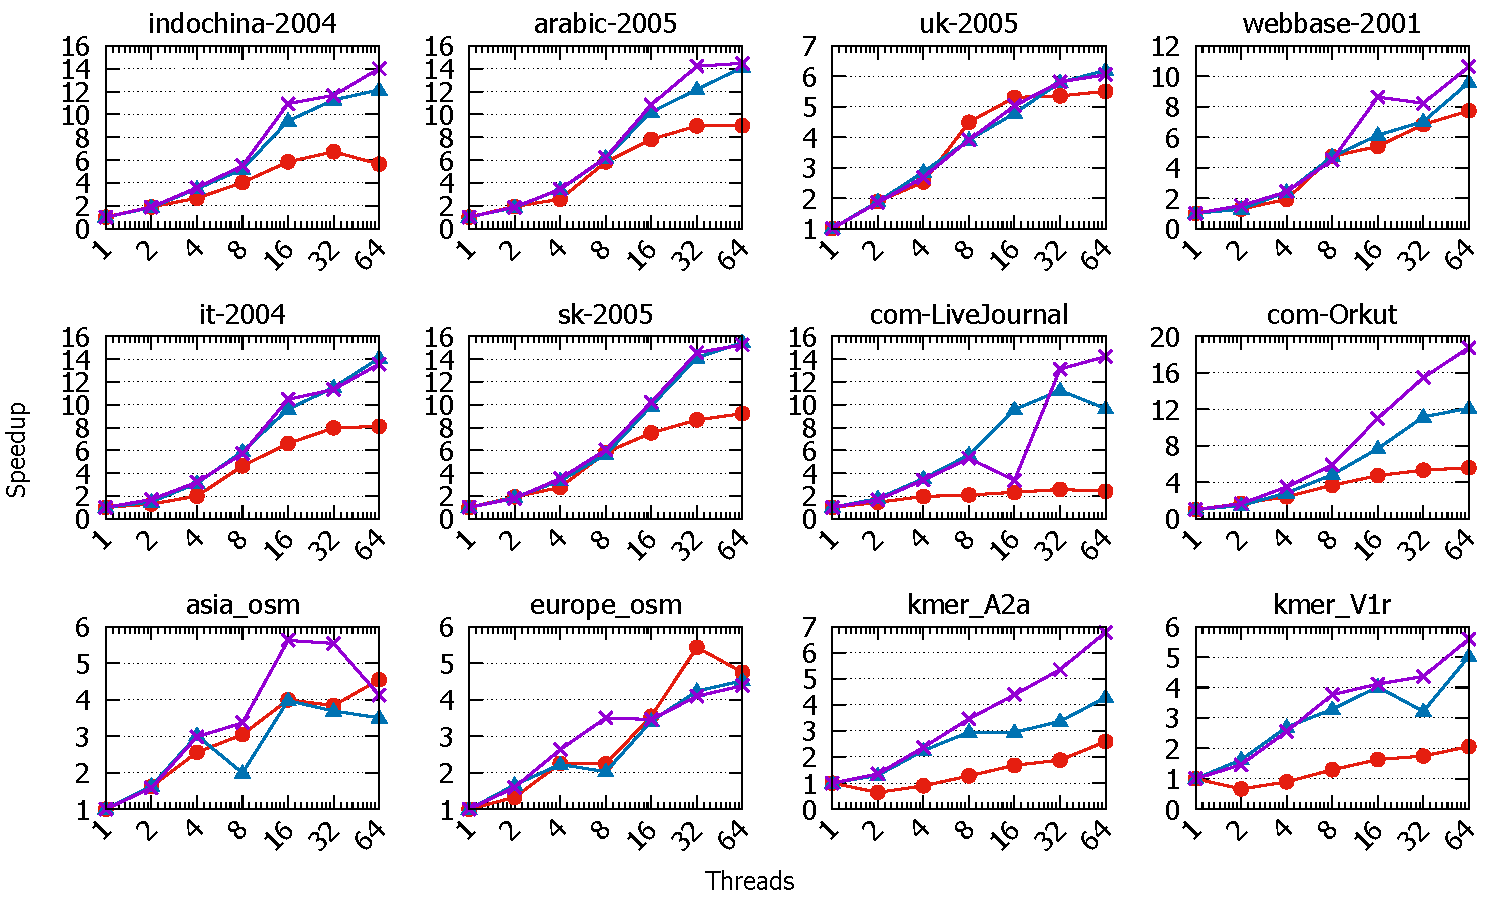
\includegraphics[width=0.58\linewidth]{out/hybrid-allss-fullx.pdf}
  }
  \subfigure[Overall result]{
    \label{fig:hybridss--am}
    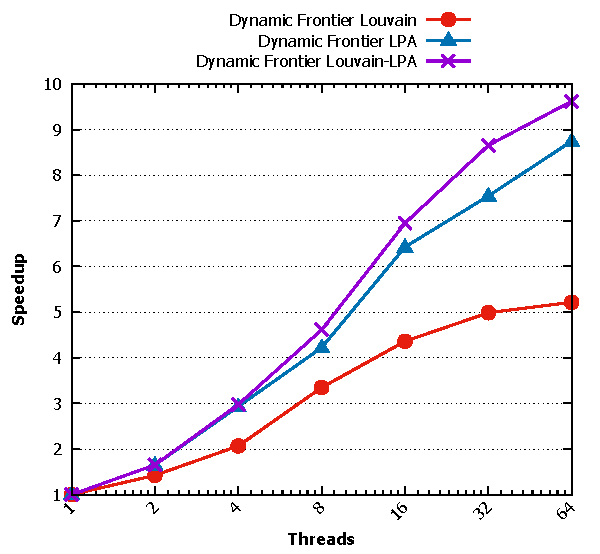
\includegraphics[width=0.38\linewidth]{out/hybrid-amss.pdf}
  } \\[-2ex]
  \caption{Speedup with respect to sequential, of \FroLou{}, \FroLPA{}, and \FroHyb{} (Algorithms \ref{alg:louvain}, \ref{alg:rak}, and \ref{alg:hybrid}) on batch updates of size $10^{-3} |E|$, with increasing number of threads from $1$ to $64$ in powers of $2$. Note that the Y-axis is linear, while the X-axis is logarithmic and captures doubling of threads naturally.}
  \label{fig:hybridss}
\end{figure*}





\subsection{Performance of Dynamic Frontier LPA (\FroLPA{}, Algorithm \ref{alg:rak})}
\label{sec:rak-evaluation}

\subsubsection{Overall Performance}

In this experiment, we study the performance of \FroLPA{} with batch updates of size ranging from $10^{-7} |E|$ to $0.1 |E|$, and compare it to \StaLPA{}, \NaiLPA{}, and \DelLPA{}. Unlike \Lou{}, none of the \LPA{} based dynamic approaches require re-initialization of communities every \verb|RESTART_LOUVAIN| batches. As discussed in Section \ref{sec:batch-update}, we employ $5$ distinct random batch updates for every batch size in order to minimize measurement noise.

Figure \ref{fig:rak--am} shows the average result of the experiment. While all approaches obtain communities of equivalent modularity, \FroLPA{} converges on average $10.0\times$ faster than \NaiLPA{} from a batch size of $10^{-7} |E|$ up to $0.01 |E|$. As shown in Figure \ref{fig:rak--all}, it has good performance on \textit{web graphs} and \textit{social networks} (graphs with high $|E|/|V|$ ratio). Note, however, that the quality of communities obtained with \LPA{} is not on par with \Lou{}.

\paragraph{Performance of Dynamic $\Delta$-screening}

Further, we note that \DelLPA{} generally fails to perform better than \NaiLPA{}. This is because it tends to mark a large fraction of the vertices as affected (see Figure \ref{fig:louvainrak-affected--rak}), and has a high associated overhead.

\paragraph{Slowdown of static algorithm}

As mentioned in Section \ref{sec:louvain-evaluation}, the uniform batches of insertions/deletions arbitrarily disrupt the original community structure, necessitating more iterations for \StaLPA{} to converge.


\subsubsection{Stability}
\label{sec:rak-stability}

Just as in Section \ref{sec:louvain-stability}, we study the stability of \NaiLPA{}, \DelLPA{}, and \FroLPA{} on random batch updates of size $10^{-7} |E|$ to $0.1 |E|$. From the results, shown in Figure \ref{fig:louvainrak-stability--rak}, we observe that \NaiLPA{} and \DelLPA{} have minimum of $95.53\%$ match with the original community memberships across all batch sizes, while \FroLPA{} has a minimum of $95.75\%$ match. This indicates that \FroLPA{} is stable.




\subsection{Performance of Dynamic Frontier Hybrid Louvain-LPA (\FroHyb{}, Algorithm \ref{alg:hybrid})}
\label{sec:hybrid-evaluation}

\subsubsection{Overall Performance}

We now study the performance of \FroHyb{}, which uses \StaLou{} every \verb|RESTART_HYBRID| batches and uses \FroLPA{} for updating communities for the remainder batches (see Sections \ref{sec:dynamic-hybrid} and \ref{sec:restart}). We do this on batch updates of size $10^{-7} |E|$ to $0.1 |E|$, and compare it with \FroLou{} and \FroLPA{} (Algorithms \ref{alg:louvain} and \ref{alg:rak}). As stated in Section \ref{sec:batch-update}, we employ five distinct random batch updates for every batch size to minimize measurement noise.

The average modularity of communities obtained by \FroHyb{} is nearly identical to that obtained by \FroLou{}, as shown in Figure \ref{fig:hybrid--am}, while obtaining a mean speedup of $7.5\times$ across batch sizes of $10^{-7} |E|$ to $0.1 |E|$. \FroHyb{} is thus an efficient and high-quality dynamic community detection approach, especially of \textit{web graphs}, as shown in Figure \ref{fig:hybrid--all}, where it significantly outperforms \FroLou{} for smaller batch updates. Note that \FroLPA{} has about the same performance, but obtains communities of lower quality.


\subsubsection{Scalability}
\label{sec:evaluation--hybridss}

Finally, we study the strong-scaling behavior of \FroHyb{} (Algorithm \ref{alg:hybrid}), and compare it with \FroLou{} and \FroLPA{} (Algorithms \ref{alg:louvain} and \ref{alg:rak}). To do this, we fix the batch size at $10^{-3} |E|$, vary the number of threads in use from $1$ to $64$, and measure the speedup of each algorithm to its sequential version. Figure \ref{fig:hybridss} demonstrates scalability of dynamic algorithms with varying thread count, measured as the time taken by the algorithm compared to the same algorithm running on one thread. Again, as indicated in Section \ref{sec:batch-update}, we employ five distinct random batch updates for each batch size to minimize measurement noise.

As shown in Figure \ref{fig:hybridss--am}, \FroLou{}, \FroLPA{}, and \FroHyb{} obtain a speedup of $5.2\times$, $8.7\times$, and $9.6\times$ respectively at $64$ threads; with their speedup increasing at a mean rate of $1.31\times$, $1.44\times$, and $1.46\times$ respectively for every doubling of threads. Also note from Figure \ref{fig:hybridss--all} that \FroHyb{} offers good speedup on \textit{web graphs} and \textit{social networks}, but does not scale well on \textit{road networks} and \textit{k-mer protein graphs} (which have a low $|E|/|V|$ ratio).




%% - https://www.reddit.com/r/intel/comments/l1kut0/what_are_some_of_the_cons_of_hyperthreading/


\section{Conclusion}
\label{sec:conclusion}
In conclusion, this study addresses the optimization of Louvain method, a high-quality community detection algorithm, in the shared memory setting. We consider 9 different optimizations, which significantly improve the performance of the local-moving and the aggregation phases of the algorithm. On a server with dual 16-core Intel Xeon Gold 6226R processors, comparison with competitive open source implementations (Vite and Grappolo) and packages (NetworKit) show that our optimized implementation of Louvain, which we term as GVE-Louvain, is on average $50\times$, $22\times$, and $20\times$ faster than Vite, Grappolo, and NetworKit respectively. In addition, GVE-Louvain on average obtains $3.1\%$ higher modularity than Vite\ignore{(especially on web graph)}, and $0.6\%$ lower modularity than Grappolo and NetworKit\ignore{(especially on social networks with poor clustering)}. On a web graph with $3.8$ billion edges, GVE-Louvain identifies communities in $6.8$ seconds, and thus achieves a processing rate of $560$ million edges/s. In addition, GVE-Louvain achieves a strong scaling factor of $1.6\times$ for every doubling of threads. Looking ahead, future work could focus of designing dynamic algorithms for Louvain to accommodate dynamic graphs which evolve over time. This would contribute to interactive updation of community memberships of vertices in real-world scenarios.


%% The acknowledgments section.
\begin{acks}
I would like to thank Prof. Kishore Kothapalli,  Prof. Dip Sankar Banerjee, Balavarun Pedapudi, and Souvik Karfa for their support.
\end{acks}

%% Bibliography style to be used, and the bibliography file.
\bibliographystyle{ACM-Reference-Format}
\bibliography{main}

\end{document}
\endinput
%% End of file.




%% NOTES:
%% - Parallelization seems to be not efficient for small batch updates.
%% - Discuss about conflicting updates
%% - 


%% TODO:
%% - Scale up the size of the graphs
%% - Move experiments to a better server
%% - Include a weak- and strong- scalabiilty plot: run the expt from 2 to 128 threads
%% - overall space planning
%% - add a few lines on novelty of the paper.
%% - table comparison of related work
%% - Include a section on preliminaries that talks about the various algorithmic ideas (Louvain, Label Propagation)

%% Workplan:
%% - KK -- Read Introduction, Related Work,
%% - Dip Sankar -- Approach -- summarize the main algorithmic ideas,
%% - Subhajit -- Results -- Plots, scalability, Dataset, experiments, implementation details,
